%%%%%%%%%%%%%%%%%%%%%%%%%%%%%%%%%%%%%%%%%%%%
%                 Preamble                 %
%%%%%%%%%%%%%%%%%%%%%%%%%%%%%%%%%%%%%%%%%%%%

% This LaTeX document uses Cameron's LaTeX template (or some form of it) which
% is ever-evolving.

% --- Requirements ---
%
% Packages from Ubuntu [required for]:
%     texlive-publishers [revtex4-1]
%     texlive-science [siunitx]

%\documentclass[a4paper]{article}
\documentclass[a4paper, 12pt, twoside]{report}
%\documentclass[
% aps,
% %prb,
% a4paper,
% showpacs,
% superscriptaddress,
% notitlepage,
% %longbibliography,
% nofootinbib,
% preprint % gives 12pt font
%]{revtex4-1}

% --- Macro dependencies ---
%\usepackage{xcolor} % Uncomment if not using bibliography links

% --- Common ---
\usepackage[left=2cm, right=2cm, top=2cm, bottom=3cm]{geometry}
\usepackage{graphicx}
\usepackage{amsmath}
\usepackage{siunitx}
\usepackage{setspace} % For line spacing
\usepackage{braket}
\usepackage{physics}

% --- More optional ---
\usepackage{tabularx} 
\usepackage{xpatch} % To patch the TOC
%\usepackage{caption} % Helps with subfigs
\usepackage{subcaption} % For subfigures
\usepackage{enumitem} % Originally to resume list

% --- Bibliography Links ---
\usepackage{hyperref}
\usepackage[dvipsnames]{xcolor}
%\hypersetup{
%	colorlinks=true,
%  linkcolor=blue,
%	citecolor=blue,
%	urlcolor=blue
%}

% --- Tikz ---
% Have to load tikz after xcolor
\usepackage{tikz}

% --- Bib title (not line) ---
\def\bibsection{\chapter*{\refname}}

% --- Macros ---
%\newcommand{\diff}{\mathrm{d}} USE \dd (physics) instead
\newcommand{\cm}[1]{\textcolor{blue}{#1}} % For my comments
\newcommand{\ph}[1]{\textcolor{green}{#1}} % Placeholders
\newcommand{\thesis}[1]{\textcolor{red}{#1}} % Placeholders
%\renewcommand{\cm}[1]{} % Uncomment to remove my comments
%\renewcommand{\thesis}[1]{} % Uncomment to remove markers for thesis work
\newcommand{\incfig}[2]{\includegraphics[width=#1\textwidth]{#2}}
\newcommand{\myeqref}[1]{eqn~\eqref{#1}}
\newcommand{\mytabref}[1]{table~\ref{#1}}
\newcommand{\myeqrefs}{eqns}
\newcommand{\myfigref}[1]{Fig.\ref{#1}}

% Chemicals
\newcommand{\CaF}{CaF}
\newcommand{\CO}{CO}
\newcommand{\YbF}{YbF}
\newcommand{\SrF}{SrF}
\newcommand{\esRb}{\textsuperscript{87}Rb}
\newcommand{\efRb}{\textsuperscript{85}Rb}
\newcommand{\ottCs}{\textsuperscript{133}Cs}
\newcommand{\RbCs}{RbCs}

% --- Units ---
% Custom units
\DeclareSIUnit\gauss{G}
\DeclareSIUnit\inch{inch}

% --- Line spacing ---
\linespread{1.5}

% --- Table of contents ---
% Patch TOC to exclude *-ed sections (default behaivour in most classes, but
% changed by design in revtex). Also exclude (sub)subsections
% Patch is quite specific to revtex
\makeatletter
%\def\l@subsection#1#2{} % Uncomment to exclude subsection
%\def\l@subsubsection#1#2{} % Uncomment to exclude subsubsection
\patchcmd{\@ssect@ltx}
    {\addcontentsline{toc}{#1}{\protect\numberline{}#8}}
    {}
    {}
    {}
\makeatother


% Uncomment and fill if using article
%\title{Early stage assessment: molecule chip}
%\author{Cameron McGarry\\ 
%Supervisors: Mike Tarbutt and Ben Sauer}

%%%%%%%%%%%%%%%%%%%%%%%%%%%%%%%%%%%%%%%%%%%%
%   Begin Document and Title/ Abstract     %
%%%%%%%%%%%%%%%%%%%%%%%%%%%%%%%%%%%%%%%%%%%%

\begin{document}

% Title page

\pagenumbering{gobble}
\begin{titlepage}
  \begin{center}
    \vspace*{1cm}
      \textbf{Design for a molecular chip trap} \\
    \vspace{1.5cm}
      \textbf{Cameron McGarry} \\
    \vspace{0.5cm}
       Supervisors: Mike Tarbutt and Ben Sauer \\
    \vspace{0.5cm}
       {Imperial College London, Department of Physics} \\
  \end{center}
\end{titlepage}

% Abstract
\chapter*{Abstract}
\cm{TODO}

%% ESA Abstract (bits)
%Quantum optical systems are promising candidates for use in a vast range of
%technologies, from metrology, to simulation, to probing the fundamentals of
%physics. But despite their high controllability and coherence times, they often
%lack scalability, requiring ungainly optical systems to function.
%
%Chip traps were introduced as a means of miniaturizing such systems. Magnetic
%traps have been formed from fields generated by wires on a substrate and
%external bias fields. This forms a robust trapping environment with very high
%field gradients. Chips are innately scalable due to their fabrication by
%well-understood standard photolithographic methods, and have been routinely
%used for experiments with atoms. Atom chips have proven to be particularly
%useful in formation of Bose-Einstein condensates. They show promise for
%coherent control, and integration with other quantum systems via coupling to
%microwave guides also integrated with the chip.
%
%With the development of new technologies for the creation of ultra-cold
%molecules, realisation of a molecule chip is now a possibility. Rotational
%states of molecules couple strongly to microwave fields, allowing the
%exploitation of cavity QED effects for use in a scalable system which can be
%integrated with other quantum architectures.
%
%% LSR Abstatract
%In this report, we present ongoing work into development of a molecule chip
%operating on a magnetically insensitive transition of \CaF{}. In particular, we
%discuss simulations that have allowed us to refine the design of the chip
%trap, and the microfabrication techniques used to build a prototype chip.
%
%Simulations of the trajectories of molecules in magnetic traps have been
%performed. These are used to analyse the trap design, and to ensure that
%loading of molecules is possible through a series of adiabatic transfers
%between magnetic potentials. The phase space acceptance of traps is presented.
%
%The microfabrication of an earlier trap design is presented. Through-mask
%electroplating has been used to construct a chip with trapping wires with
%heights of \SI{3}{\micro\meter}. This is much taller than would be possible
%with conventional photolithography methods, and will allow for high currents to
%be carried on chip, thus forming deep magnetic traps for our molecules.

\clearpage

% TOC
\tableofcontents
\clearpage

% Numbers on
\pagenumbering{arabic}
%NOTE This must be manually set so that numbering starts on title page
\setcounter{page}{4} 

%%%%%%%%%%%%%%%%%%%%%%%%%%%%%%%%%%%%%%%%%%%%
%                Body Start                %
%%%%%%%%%%%%%%%%%%%%%%%%%%%%%%%%%%%%%%%%%%%%

\thesis{Roll atomic and molecular chip traps into the intro}

\chapter{Introduction}
% Could have mentioned ion chips. Reviews:
%\cite{RevModPhys.62.531}
%\cite{Romaszko2020} (mostly chips?)

One of the reasurring things about new experiments with ultracold molecules is
that a lot of what researchers may wish to accomplish has an
already-accomplished analogue in the well-established field of cold atoms. On
the whole, researchers of molecules have been able to foolow this existing
roadmap, from laser slowing, to magneto-optical trapping, to optical dipole
trapping; all of which will be discussed in the next section. A next obvious goal may
be evaporative cooling and the creation of a Bose-Einstein condensate, but
there is another convenient and useful tool of cold atom experiments whose
molecular parallel has yet to be realised.

This tool is the atom chip which, we will see below, has proven to be of great
use as a robust, compact and portable device for cold atom experiments. A
molecular counterpart could prove to be equally invaluable, and offer
improvements on existing atom chips, by allowing strong coupling to microwave
fields on the chip, including the realisation of a cavity quantum
electrodynamics system. Such a device was originally proposed by Andre et
al.~\cite{Andre2006}, as a `coherent all-electrical interface between polar
molecules and mesoscopic superconducting resonators.'

This chapter provides an outline as to why a molecule chip trap for ultracold
molecules is a desirable goal, starting from a review of cold atoms, to atom
chips and then cold molecules. I will then summarise the motivation for a
molecule chip and outline the structure of the thesis.

\section{Ultracold atoms}

Laser cooling of atoms is a developed field, with the 1997 Nobel Prize in
Physics having been awarded to Cohen-Tannoudji, Chu and Phillips for
`development of methods to cool and trap atoms with laser
light'~\cite{RevModPhys.70.721}. The subject is reviewed in various texts, with
the canonical reference being Metcalf and van der Straten~\cite{Metcalf1999}.
Here I will give a brief qualitative overview of the topic and its many
applications in modern physics, which include quantum: information,
communication and metrology. Further details on these cooling mechanisms are
given in section~\ref{theory:cooltrap}.

In a typical laser slowing experiment, the forward velocity of a beam of atoms
is reduced by resonant, counter-propagating laser light. An atom can scatter
a photon from the laser, upon re-emission the photon has no preferred
direction of travel. Over a large number of photon scatters this results in a
net reduction in the forward velocity of the atoms~\cite{PhysRevLett.40.1639}.
This principle of slowing with radiation pressure was first observed by
Wineland et al.~\cite{PhysRevLett.40.1639} in \Mg{} ions, but one of the key
goals of laser slowing was to sufficiently reduce the velocity of a beam of
neutral atoms (produced in, for example, an oven) to sufficiently low
velocities for trapping. 

To achieve this it is essential to account for the change in the resonant
frequency of the atoms due to the Doppler shift that occurs as the atom's
velocity is reduced. Phillips and Metcalf~\cite{PhysRevLett.48.596} were able
to achieve this for \Na{} atoms by the Zeeman slowing technique, where a
changing magnetic field across the beamline is used to ensure the relevant
transition is always resonant with the light. Later the same group would
achieve the same effect by chirping the frequency of the
light~\cite{Prodan1984}, so that the light is sufficiently red-shifted to be
resonant with the atoms as they slow down.  Such experiments must take place
under ultra high vacuum to prevent loss by collisions with a background gas.

Magnetic trapping of the atoms soon followed, with the slow atomic beam
directed into a quadrupole field generated by current-carrying coils. The atoms
could be pumped into a weak-field seeking state, and trapped in the field
minimum~\cite{PhysRevLett.54.2596}. The next key development was the
implementation of the magneto-optical trap (MOT) where atoms were confined by a
quadrupole magnetic field and red-detuned laser light incident from every
direction. This scheme is designed so that atoms that are away from the trap
centre experience a Zeeman shift that brings them into resonance with the
light. The polarisations are then chosen so that the atom will preferentially
scatter photons from the beam that will result in a restoring force towards the
trap centre. The benefit of this over the magnetic trap being that as well as a
position-dependent restoring force, there is a velocity-dependent damping to
reduce the atoms' temperature. This was first implemented by by Raab et
al.~\cite{PhysRevLett.59.2631}, also in \Na{}, although subsequently many
different species have been laser-cooled and confined in a MOT.

Due to the stochastic nature of Doppler-cooling, there is a fundamental limit
on the lowest temperature that can be achieved using just the Doppler slowing
mechanism. This can be reached by turning the magnetic field of the MOT off,
leaving just the red-detuned laser beams to form an optical molasses. Early
implementations of this scheme found that in fact, anomalously low temperatures
were reached in a molasses~\cite{Lett1988}. This was eventually explained by
Dalibard et al.~\cite{Dalibard:89} as being due to sub-Doppler cooling
mechanisms, which rely on polarisation gradients set up in the light field.
This reduced the atom temperature to the so-called recoil limit, which is
related to the energy imparted by a single photon scatter.

It is possible to cool beneath even the recoil limit by evaporative cooling,
where the hottest atoms are ejected from the trap. The remaining atoms
thermalise at a lower temperature than the original cloud. This technique was
employed by Anderson et al.~\cite{Anderson198} to cool \esRb{} to sufficiently
low temperature and density to form a Bose-Einstein condensate (BEC). Another
now-popular method of producing high-density atomic clouds is the optical
dipole trap~\cite{Chu1986}, where atoms are confined by intense,
far-off-resonant light. Atoms in such a trap are confined by the a.c.\ Stark
shift, which creates an attractive potential towards the region where the
light's intensity is greatest.

For a sufficiently tight optical dipole trap, an optical tweezer is formed,
where a single atom can be trapped and easily manipulated by controlling the
light~\cite{Schlosser2001}. A series of tweezer traps can be used to form a
lattice of traps~\cite{Schlosser2001}, with individually-trapped atoms able to
interact with each other by dipole-dipole interactions. A lattice can also be
formed in a standing wave optical trap (SWOT), where light reflected from a
surface creates a series of local field maxima for trapping of
atoms~\cite{Wu2017}.

With the ability to reliably create low-temperature atomic clouds (or even a
single atom) confined in traps and lattices, comes the ability to create
quantum devices for simulation, communication and metrology, with promises of
future applications in quantum computing. Coherent control of atoms in optical
lattices for simulation has been demonstrated~\cite{Schafer2020}, and optical
lattice clocks have become the cutting edged in
timekeeping~\cite{PhysRevX.8.021036}. There are numerous examples of atoms
being used for precise sensing, for example, acceleration~\cite{Chen2019}
including gravity~\cite{Stray2022}. Cold atoms can also be employed to
explore fundamental physics, such as the search for dark
matter~\cite{Wcislo2018}. Future experiments also plan to utilise cold atoms
for new gravitational wave detectors operating in frequency bands that are
inaccessible to existing detectors~\cite{Badurina_2020}.

These experiments, and those like them, have been made easier by technological
developments such as atom dispensers, which remove the need to cool
a hot beam of atoms, and vapour cells, which can entirely remove the
need for a complicated vacuum system. This has lead the way to miniaturisation
and scalability of cold atom experiments, which is an active field of research.
The complexity of these experiments can be further reduced by using, for
example pyramid~\cite{Lee:96}, mirror~\cite{Reichel1999, 4797887} or
grating~\cite{Nshii2013} MOTs, where some of the MOT light beams are produced
by reflection or diffraction from a surface. These are strongly linked to the
main focus of this thesis: the chip trap.

\section{Chip traps}

The chip trap was proposed as a mechanism for studying atoms in very
high-gradient magnetic traps~\cite{PhysRevA.52.4004}, but it has evolved into a
useful tool for miniaturised and robust cold atom experiments. These can be
integrated with, for example, microwave components, to form hybrid quantum
systems. Further details will be presented in section~\ref{theory:chips}, but
here I will give a brief overview of the operating principles and history of
atomic chip traps.

We have already discussed the idea of trapping atoms in a quadrupole magnetic
field, however in the above-described experiments the fields were generated by
macroscopic current-carrying coils. It is also possible to generate magnetic
traps from the field of a wire combined with a homogeneous bias field. In a
chip trap experiment, the wires are positioned on the surface of a substrate,
and can be made very small (on the scale of a few microns) by the use of common
microfabrication techniques. Various microscopic atom traps were pioneered by
by H\"ansch and Zimmermann at the Max Planck Institute of Quantum Optics (MPQ)
and T\"ubingen~\cite{PhysRevLett.80.1634, PhysRevLett.81.5310}, as well as in
Harvard~\cite{Drindic1998}. This was followed by work in Innsbruck, where \Li{}
atoms were guided using a two dimensional trap formed with a free-standing
wire~\cite{PhysRevLett.82.2014}. 

The first true chip traps, operating in three dimensions were reported by the
MPQ group~\cite{Reichel1999}, who also implemented a mirror-MOT for loading
\esRb{} into their traps. This was shortly followed by developments in
controlling and guiding \Li{} atoms trapped above a chip's
surface~\cite{Folman2000} from Innsbruck.
%
Atom chips were soon found to be a robust tool for cold atom experiments,
including the production of BECs, with groups from the Ludwig Maximilian
University of Munich and T\"ubingen both reporting \esRb{} BECs at the same
conference in 2001~\cite{Hansel2001, dtt2001}. Since then atom chips have been
used to investigate lower dimensional gasses, as reported in
\inlinerefs{PhysRevLett.116.030402, Hofferberth2007, Yuen2015}, and have found
uses in various other experiments as a convenient method of preparing cold
atomic clouds~\cite{PhysRevLett.104.073604}.
%
This includes experiments creating non-classical spin-squeezed states (see
chapter~\ref{squeeze}), implementing magnetic lattices~\cite{Gerritsma2007} and
performing interferometry~\cite{Wang2005}.

2004 saw the first implementation of an on-chip Michelson interferometer, based
on the creation, splitting and guiding of BECs all on a chip. In the same year,
prospect of integrated atom chip devices was fully realised at the National
Institute of Standards and Technology, where a compact and portable atomic chip
clock was developed~\cite{Knappe2004} based on the hyperfine transitions in
\Cs{}. This has since become a commercial product with uses across a variety of
fields, such as military and space science~\cite{RAMIREZMARTINEZ2011247}
including an atom chip experiment conducted on board the International Space
Station~\cite{Frye2021}.

Also in 2004, it was demonstrated by the MPQ group that coherence times of
around \SI{1}{\second} could be achieved for \esRb{} atoms held in a chip trap
within \SI{100}{\micro\meter} of the surface~\cite{Treutlein2004}. In this
experiment microwave fields were used to drive hyperfine tranisitons in the
molecules, with the microwave radiation delivered from an external source. This
was soon extended to experiments where the microwaves were delivered by on-chip
microwave components built on a two-layer device~\cite{Treutlein2008,
Boehi2009}, with a view to develop a microwave trap and perform quantum
gates entirely on-chip.

The work of the Munich group built towards coherent control of an atom coupled
to on-chip microwaves, however a more ambitious goal is the coupling of an atom
to a microwave cavity, which can lead to powerful control over the spin system
by leveraging the effects of cavity quantum electrodynamics. One requirement of
this is so-called strong coupling between the microwave photons and the atomic
transition, which is challenging due to the comparatively small transition
matrix element of the hyperfine transitions in the atoms, and the need for a
high quailty microwave cavity. The latter of these, as we will discuss in
chapter~\ref{mws}, requires the use of superconducting microwave components.

A superconducting atom chip is an attractive idea, since as well as the
potential for low-loss microwave components, sueprconducting wires can produce
deeper magnetic traps. The first such device was produced in first realised by
Haroche's group in Paris in 2006~\cite{Nirrengarten2006}, with a BEC on a
superconducting chip following in 2008~\cite{Roux2008}. Similar superconducting
wire traps were used to investigate the Meissner
effect~\cite{PhysRevLett.101.183006}, and subsequent development of these
superconducting atom chips lead to full quantum control of an atom cloud held
in place above a superconducting microwave resonator~\cite{Bernon2013}. Here
the resonator was designed to be off the atomic resonance, so that the internal
state of the trapped atoms were unaffected by its presence. Of additional note
in this paper is the loading scheme used for the chip -- an optical tweezer is
used to bring the atoms from a room-temperature environment to within
\SI{400}{\micro\meter} of the chip surface, before being transferred to
surface-based microtraps.

A later experiment~\cite{Hatterman2017} would see the coupling of atoms to the
microwave resonator, realising a hybrid atom-microwave system, and the
investigation of microwave cavity quantum electrodynamics. Rabi oscillations
between hyperfine transitions could be driven, but strong coupling was not, and
has not been achieved. It has been possible to couple atoms strongly to, for
example monolithic microresonators~\cite{Aoki2006}, but only in freefall, not whilst
trapped. Other efforts to reach this strong coupling regime come from Hogan's
group, who use Rydberg atoms, utilising the increased electric dipole moment of
the transition (typically a factor of 1000 larger than for ground-state atoms)
to achieve stronger coupling~\cite{PhysRevLett.124.193604}. Again, such
experiments are performed with atoms that are in flight, and in this case
travelling at supersonic speeds.

An improvement to such experiments would be to confine the atom close to the
microwave field, near the anti-node of the resonator to maximise the coupling
strength. However, another potential method is to use a molecule with high
electric dipole moment instead of a Rydberg atom. Recent advances in the
laser-cooling and trapping of diatomic molecules make these an exciting
prospect for implementing a microwave cavity QED device, as was originally
proposed by Andre et al.~\cite{Andre2006}. In the next section we will briefly
review this field, before further outlining the prospects for a molecule chip
trap.

\section{Ultracold molecules}

There are a number of potential benefits that can come from cooling molecules
rather than atoms. As already mentioned, molecules can have a permanent
electric dipole moment in their ground state, allowing for strong dipole-dipole
coupling in a lattice, or to external fields.
%
Molecules also allows the investigation of fundamental physics, such as the
measurement of the electron's electric dipole moment, measurement of
which has helped to eliminate particle physics theories that go beyond the
standard model~\cite{ACMEreview}.

The energy structure of molecules is far richer than that of atoms; a diatomic
molecule will have both vibrational and rotational energy levels, which can be
leveraged for novel imaging schemes, strong coupling to microwave transitions,
amongst other applications. However these introduce additional complications
that make experiments with ultracold molecules more challenging than their
atomic equivalents.

There are two main schools of ultracold molecule experiments, in the first of
these gases of cold atoms are used to synthesise cold molecules, usually by
association by Feshbach resonance~\cite{Moses2017,PhysRevA.89.033604}. However
in this thesis we will focus on the direct cooling of hot diatomic molecules.
The first experiment to successfully trap molecules was reported by Weinstein
et al.~\cite{Weinstein1998}, who created calcium monohydride (\CaH{}) molecules
by laser ablation, and then to below the depth of a magnetic trap by buffer-gas
cooling. In this technique, an inert buffer gas is used as an intermediary to
thermalise the molecules with a cold copper cell typically held at a few
kelvin.
%
An alternative technique to slow a beam of molecules was developed in Gerard
Meijer's group, who leveraged the permanent electric dipole moment of molecules
used Stark deceleration to first slow a beam of carbon
monoxide~\cite{Bethlem1999}, and later to slow then electrostatically trap
ammonia in both a quadrupole trap~\cite{Bethlem2000} and a storage
ring~\cite{Crompvoets2001, Crompvoets2005}. However these methods produce
molecules that are orders of magnitude warmer than the atoms produced by laser
slowing.

Buffer gas cooling became a staple of cold molecule experiments, being
routinely used in the production of slow, high-flux molecular
beams~\cite{Maxwell2005, Patterson2007, Barry2011}.  Optical cycling in a
diatomic molecule with the potential of laser slowing was first seen using
strontium monofluoride (\SrF{}) by DeMille's group~\cite{Shuman2009}. To
account for the more complex energy structure of the molecule, additional
lasers were used to repump the molecule from states that were dark to the
cooling transition.  Despite this difficulty, the DeMille group had soon enough
applied the technique to achieve laser-slowing~\cite{PhysRevLett.108.103002}
and eventually an \SrF{} MOT~\cite{Barry2014, PhysRevLett.116.063004}. The
initial report boasted temperatures less than \SI{1}{\milli\kelvin} and there
was scope to reduce this further.

Alongside the development of laser-cooling \SrF{}, there have been developments
in the laser-cooling of various other molecules, notably ytterbium monofluoride
(\YbF{}) and calcium monofluoride (\CaF{}), the latter being the main molecule
of focus in this thesis. YbF has been used in various experiments to measure
the electric dipole moment of the electron, and it is hoped that laser-cooling
could be a method for further reducing the associated uncertainty~\cite{Fitch2020}. Meanwhile, \CaF{} shows promise as a molecule of
itnerest for investigating quantum information and the fundamentals of quantum
chemisty. Laser-slowing of \CaF{} was first observed in the Centre for
Cold Matter (CCM) at Imperial College London~\cite{PhysRevA.89.053416}, where a
supersonic beam was slowed by \SI{20}{\meter\per\second} using a chirped beam of
light. The \CaF{} experiment was further developed with the implementation of a
buffer gas source for \CaF{}~\cite{Truppe2018}, with further developments in
laser slowing coming from both CCM~\cite{Truppe2017a} and the Doyle group in
Harvard~\cite{0953-4075-49-17-174001}.

A \CaF{} MOT was first reported by the Harvard
group~\cite{PhysRevLett.119.103201}, followed shortly by
CCM~\cite{Williams2017}. Both experiments taking slightly different approaches
to avoid the pumping of molecules into dark states, using r.f.\ switching and
dual-frequency techniques respectively. The \CaF{} MOT has opened the door to
experiments with large clouds of \CaF{} molecules, with today's MOTs capable of
loading $\sim10^5$ molecules~\cite{PhysRevLett.119.103201}. The temperatures of
these clouds can be further reduced to below the Doppler
limit~\cite{Truppe2017, PhysRevLett.123.033202} and can then be further trapped
and controlled by some of the same techniques already discussed above for
atoms. This includes confinement in magnetic~\cite{WilliamsMagnetic2018} and in
a lattice~\cite{Anderegg2019a}. Futher cooling schemes such as transverse
cooling (similar to that seen for \YbF in \inlineref{Alauze2021}) and
Zeeman-Sisyphys cooling have been demonstrated\cite{Fitch2016,
PhysRevLett.127.263002}.  Combining these various schemes with ongoing research
into collisions with atoms~\cite{PhysRevLett.126.153401} and sympathetic
cooling could see even lower \CaF{} temperatures achieved in the near future.

\CaF{} has shown to have promise in quantum information and simulation, with
coherent control in a magnetic trap having been
demonstrated~\cite{WilliamsMagnetic2018, Blackmore_2018} with coherence times
of over \SI{1}{\second} plausibly
achievable~\cite{PhysRevLett.124.063001}.Coherent control of the molecule has
also been demonstrated in a dipole trap~\cite{PhysRevLett.127.123202}, showing
that there is significant potential for the implementation of quantum
simulations and computing. Further novel schemes for molecule-based quantum
information have been proposed, such as those described for topological quantum
computing in \inlineref{Micheli2006} or for the implementation of qudits in
\inlineref{Sawant_2020}.

Another topic of interest is collisions between cold molecules and cold atoms.
This has recently been observed in sodium lithium molecules by Son et
al.~\cite{son2019collisional}, and in \CaF{} in CCM~\cite{Jurgilas2021,
JurgilasPRL_2021}. The thermalisation of molecules with atoms could lead to
further temperature reduction by sympathetic cooling, which may be enhanced in
a dipole trap. It also paves the way for investigations into quantum chemistry
at a very fundamental level. Recent research into the production of polyatomic
MOTs by the Harvard group~\cite{DoylePolyatomic2022} will no-doubt also play an
important role in such investigations.

To summarise, research into ultracold molecules is rapidly developing, with
methods for producing cold, dense clouds of diatomic molecules already
available. The rich energy structure, and permanent electric dipole moment of
molecules makes them a promising candidate for use in quantum information,
communications and sensing experiments including in chip-based devices.

\section{Molecule chip trap}

We have seen in the above discussion that ultracold molecules can be a useful
tool in quantum information and simulations. Further, recent developments in
cooling techniques mean that we are now able to produce dense clouds of
molecules such as \CaF{}, which exhibit long coherence times in magnetic traps.
Various techniques that have been applied to cold atoms have been equally
successfully applied to cold molecules, but a conspicuous absence in the
preceding discussion is a chip trap for ultracold molecules.

Such a device is of significant interest, since the various capabilities of
atom chips: a robust and stable architecture for quantum experiments could
prove extremely useful when applied to cold molecules. Diatomic molecules, such
as \CaF{} have now been laser-cooled and magnetically confined. In modern
systems dense clouds can be created, which are suitable for loading into
magnetic chip traps (see chapter~\ref{sim}). Further, polar molecules can be
contained in electrostatic traps, which could be leveraged to construct traps
similar to existing ion chip traps~\cite{Andre2006, Romaszko2020}. Such devices
are inherently scalable, with the ability to constrain multiple molecules at
various sites across the chip surface. They can then be transported by changing
the electric potentials, which simply amounts to changing the voltages on
trapping electrodes.

Another benefit of a molecule chip system is that the rotational transitions in
a diatomic molecule can couple very strongly to microwave fields, much more so
than the hyperfine transitions in atoms. Andr\'e et al.~\cite{Andre2006}
propose that building a molecule chip with integrated microwave guides, similar
to equivalent atom chips reported in \inlineref{Nirrengarten2006} could provide
access to powerful tools for quantum information and communication. Amongst
these are the ability to carry out a non-demolition measurement of the molecule
state. This, along with the ability to drive microwave transitions using the
guide, allows the device to be totally self contained -- once molecules
are loaded all interactions can be performed electrically. The long-lived
rotational states of \CaF{} make this molecule a promising candidate such a
device.

Along with readout, strong coupling to a resonator could allow for the
implementation of a novel sideband cooling scheme to reduce the molecule's
motional energy to the ground state of the trapping potential. It would also be
possible to couple neighbouring trapping sites using the resonator as a bus.
Similarly it may be possible to extend the interaction to longer ranges, since
photons can be used as flying qubits to couple quantum mechanical systems over
long distances. The schemes mentioned in this section will be explored further
in chapter~\ref{mws}.

There has been some work investigating molecules trapped close to chips, mainly by
the Meijer group, who have designed and implemented microfabricated Stark
decelerators~\cite{Meek2008}, and even trapped molecules on a
chip~\cite{Meek2009}. However, similar to their other work, these molecules are
much hotter than can be achieved with laser-cooling.

This thesis describes the work that has been undertaken in CCM to build a
microfabricated chip trap for \CaF{} molecules at ultracold temperatures. I
will outline a design inspired by existing atom chips, and the proposals in
\inlineref{Andre2006}. This design will provide a stepping stone towards more
advanced devices, which will be able to implement the various schemes described
above. It will integrate with the existing experiment, and take advantage of
the properties of \CaF{}, including the long coherence times of rotational
transitions that can be achieved in magnetic traps.

\section{Structure of the thesis}

In chapter~\ref{theory} we will introduce key background theory: 
laser-cooling of simple systems, the operation of chip traps, and the physics
of diatomic molecules. Next chapter~\ref{overview} gives an overview of the
existing \CaF{} experiment, as well as some particulars of the laser-cooling
methods used specifically for \CaF{}. Here we will also outline the new chip
experiment, and how it will integrate with the existing apparatus. We have
demonstrated the loading procedure for the trap with simulations, and these are
presented in chapter~\ref{sim}.

We microfabricated chip traps, as will be discussed in chapter~\ref{fab}, and
then loaded these into a vacuum chamber for initial testing. This included
testing that the current capcity of the trapping wires was as expected, that
ultra-high vacuum could be reached, and that it will be possible to image
molecules without too much background scatter created by the chip. These tests,
and a scheme to reduce the background scatter are discussed in
chapter~\ref{experiment}. Chapter~\ref{mws} describes how a microwave guide and
resonator can be implemented as part of the experiment, as well as the
behavoiur of a single molecule coupled to a microwave cavity. We will extend
this idea for ensembles of molecules coupled to a cavity in
chapter~\ref{squeeze}, where I propose a scheme to use a quantum non-demolition
measurement to create a spin-squeezed state in such an ensemble. Finally,
chapter~\ref{outlook} describes the future prospects for this project.


\chapter{Atomic and molecular chip traps}
\label{chiptraps}
\cm{
 Take-away points:
   Magnetic trap
   How to get CPW on (Bohi)
   MTT + big U to load is viable
   Required PSD???
 }

At the time of the original molecule chip proposal~\cite{Andre2006}, atom chips
had been loaded using a MOT as a source~\cite{Reichel1999, Ott2001}, however a
molecule MOT had not yet been \cm{built (better word choice?)}, and there was no
credible source of loading a chip of this type.\footnote{Stark declerator
molecule chips would be developed shortly after~\cite{Meek2009}, but Andr\'e et
al. presented no method of loading their chip design with the required phase
space density.}  

As discussed above, the field of cold molecules has now developed significantly.
These developments have made the implementation of a molecule chip \cm{feasible
(better word choice?)}. In
this section, we will review the state of chip trapping, including work on atom
chips and these supporting technologies.

In developing the molecule chip, we have been able to draw upon the
well-developed field of atom chips to inform our design choices. Let us consider
three different aspects of chip design: trapping on the chip, loading into this
trap, manipulation of trapped atoms or molecules.
\cm{Here I define three key features, I should endeavour to address each of
them. Perhaps as separate (sub)sections. I may even want to introduce this more
explicity/ formally further above.}

The Andr\'e proposal~\cite{Andre2006} suggests the use of an electrostatic trap
to contain the molecules, however this is not the only option available. In
fact, magnetic trapping of atoms is much more widely explored~\cite{2011Ac},
and the discovery of magnetically insensitive transitions in \CaF{} makes this a
promising choice for a molecule chip. As such we will focus in this section on
magnetostatic trapping of atoms above a chip.

\subsection{Magnetic trapping}
\label{chiptraps:magentic}

\cm{TODO: theory of macroscopic, then feed into miiatrurising and hence the next
section}

\cm{Talk about IP s . QP and spin flip, including further discussion about
theory of spin flip (majorana) losses and how much we can get away with (to be
expanded on further below for Z wire/ dimple traps where we get really small.}

\subsection{Wire traps}
\label{chiptraps:wiretraps}

The basic principle of a magnetic wire trap is explained in Reichel et
al.~\cite{Reichel1999} As illustrated in \myfigref{chiptraps:fig:reicheltrap} a
field zero can be created from the magnetic field of a straight wire, carrying
current $I$, and an external bias field. This is a two-dimensional trap
\cm{2D?}, with a zero running parallel to the wire. The bias field's direction
must oppose the direction of the wire field. To form the zero at some height $h$
above the wire the bias field must completely cancel the wire field at that
point, so that \cm{Need to check B or B-tilde..}
%
\begin{equation}
  B = \frac{\mu_0 I}{2\pi h}.
\end{equation}
%
As with other magnetic traps, atoms (or molecules) can be optically pumped into
weak-field seeking states such that they favourably occupy the region surround
the trap minimum.~\cite{Metcalf1999}

\begin{figure}
  \includegraphics[width=0.75\textwidth]{./figs/chiptraps/reicheltrap.pdf}
  \caption{The combination of the magnetic field due to a straight wire and a
  constant bias are shown to produce a zero, forming a two-dimensional trap for
  weak field seekers. This is the basic principle underlying all magnetic wire
  traps. Reproduced from Reichel et al.~\cite{Reichel1999}
  }
  \label{chiptraps:fig:reicheltrap}
\end{figure}

\cm{I should have described QP/IP difference above}
Such a field will form a two-dimensional trap for weak-field seeking particles.
To achieve a three-dimensional trap, we can overlay an additional wire,
carrying a smaller current than the first such that there is now some component
of magnetic field along the axis of the original trap. Applying a bias along
this axial direction will re-introduce a field minimum, forming a three-dimensional
\emph{dimple trap} shown in \myfigref{chiptraps:fig:dimpletrap}.~\cite{2011Ac}
Since the trap centre is now in general a field minimum rather than a
zero, it is a Ioffe-Pritchard trap.

\begin{figure}
  \includegraphics[width=0.75\textwidth]{./figs/chiptraps/dimpletrap.png}
  \caption{The field of a straight wire trap (current $I_0$ is perturbed by a
  second wire carrying a current $I_1 \ll I_0 $ and accompanying bias
  ($B_{b,x}$). The resulting field forms a three-dimensional dimple trap.
  }
  \label{chiptraps:fig:dimpletrap}
\end{figure}


% Maths for the traps, freq. grad. etc.
The trapping field of the dimple trap close to the centre can be described in
terms of the usual Ioffe-Pritchard equation~\cite{Foot2005}
%
\begin{equation}
  \mathbf{B} = B_0 \begin{bmatrix} 1 \\ 0 \\0 \end{bmatrix}
               + B' \begin{bmatrix} 0 \\ -y \\ z \end{bmatrix}
               + \frac{B''}{2} \begin{bmatrix} 
                  x^2 - \frac{1}{2}(y^2 + z^2) \\
                  -xy \\
                  -xz
               \end{bmatrix},
\end{equation}
%
where we have chosen the origin to be the trap centre (not to be confused with
the centre of the dimple wires). In this case, the field gradient and curvature
are
%
\begin{equation}
  B' = \frac{\mu_0 I_0}{2\pi h^2}
\end{equation}
%
and
%
\begin{equation}
  B'' = \frac{\mu_0 I_1}{\pi h^3}
\end{equation}
%
respectively. The field at the trap centre is
%
\begin{equation}
  B_0 = \widetilde{B}_x + \frac{\mu_0 I_1}{2\pi h}
  \label{chiptraps:eqn:bias}
\end{equation}
%
where $\widetilde{B}_i$ represents the bias field applied in the $i$ direction.
The trap frequencies are given by
\begin{equation}
  \omega_x = \sqrt{\frac{\mu_m}{m}B''}
  \label{chiptraps:eqn:axisfreq}
\end{equation}
and
\begin{equation}
  \omega_\perp = \sqrt{\frac{\mu_m {B'}^2}{m B_0}}
  \label{chiptraps:eqn:transfreq}
\end{equation}
where $\mu_m$ is the magnetic moment of the trapped particle (for our \CaF{}
transitions $\mu_m \approx \mu_B$, the Bohr magneton), and we have taken $x$ to
be the axial direction (aligned with $I_0$).~\cite{2011Ac} We can estimate the
expected frequencies that we would expect to achieve based on the current and
trapping height.

\cm{I probably want to go through this in a lot more detail including the
maths. This is all in the notebook that Ed Hinds gave me to start with.} A
typical final\footnote{Greater intermediary trapping heights are used as part of
the loading procedure.} trapping height will be around \SI{10}{\micro\metre}.
This allows on-chip microwave fields to interact with trapped atoms without
introducing any energy shifts  or significant attractive force acting on the
molecule from the Casimir effect or Van der Waals force.\footnote{Trapping
beneath this height could allow investigation of these effects on a quantum
scale and is in itself a goal of atom chip
trapping.~\cite{PhysRevA.56.R3350}}~\cite{2011Ac}

\cm{Probably want to expand this similar to for height}
The current that can be achieved in the chip will be limited by thermal
properties of the final chip design as will be discussed in
section~\ref{experiment:multilayer}. Typical achievable currents are estimated
to be around \SI{60}{\milli\ampere}. 
Using \myeqref{chiptraps:eqn:transfreq} and
\myeqref{chiptraps:eqn:axisfreq} we can therefore anticipate trapping frequencies
for \CaF{} of
%
\begin{align}
  \omega_x &= \SI{5e4}{\radian \per \second} \\
  \omega_\perp &= \SI{1e5}{\radian \per \second}.
\end{align}
%
\cm{Need to check reasonable value for $B_0$}
Where we have assumed a minimum value of $B_0 = \SI{1}{\gauss}$ has been chosen.
These figures are in line with what we would normally expect from a wire
trap.~\cite{2011Ac}

The trap depth is well-approximated by the energy associated with the bias
field. For a trap at height \SI{10}{\micro\metre} this gives a typical trap
depth on the order of a few tens of millikelvin.~\cite{2011Ac}

Other variations on the wire trap are possible. Running two perturbing wires
across one axis (with currents $I_1$ and $I_2$) will form an H-trap, shown in
\myfigref{chiptraps:fig:trapvariations}. Here the minimum will exist between the
two perturbing wires. Note that depending on the relative signs of $I_1$ and
$I_2$ it is possible to form either a Ioffe-Pritchard (currents parallel) or a
quadrupole trap (currents anti-parallel). Approximations of these shapes can be
formed by bending a single wire to create the axial confinement, forming either
a Z-trap (Ioffe-Pritchard) or U-trap (quadrupole), both also shown in
\myfigref{chiptraps:fig:trapvariations}. \cm{I should really show the fields
that are generated, as well as the bias fields required, a coordinate system and
follow up on expected Majorana losses properly below.}

\begin{figure}
  \centering
\begin{tikzpicture}
  % H
  \draw[thick, ->] (-6,0) -- (-3,0);
  \node at (-2.75,-0.25) {$I_0$};
  \draw[thick, ->] (-5.5,-3) -- (-5.5,3);
  \node at (-5.15, 3) {$I_1$};
  \draw[thick, ->] (-3.5,-3) -- (-3.5,3);
  \node at (-3.15, 3) {$I_2$};
  \node at (-6.5, -2.5) {(H)};
  % U
  \draw[thick, ->] (-1,3) -- (-1,0) --(1,0) -- (1,3);
  \node at (1.35,3) {$I$};
  \node at (-1.5, -2.5) {(U)};
  % Z
  \draw[thick, ->] (3,-3) -- (3,0) --(5,0) -- (5,3);
  \node at (5.35,3) {$I$};
  \node at (2.5, -2.5) {(Z)};
\end{tikzpicture}
  \caption{
    A top-down view of the wires forming an H, U and Z trap. The H trap has
    three independent currents, $I_0$, $I_1$ and $I_2$; usually the magnitudes
    of $I_1$ and $I_2$ will be the same, however their relative signs can be
    chosen to form either a quadrupole ($I_1 = -I_2$) or Ioffe-Pritchard ($I_1 =
    I_2$) trap. Note that these cases correspond to the U and Z wires
    approximating the currents through the H wire respectively. The bias fields
    requisite for trapping are not shown.
  }
  \label{chiptraps:fig:trapvariations}
\end{figure}

\cm{
``Frequencies for the other trap types can be calculated numerically, but the
above figures are presented as a representative example of what can be expected
from a wire trap.'' \\
%
Maybe I should actually do this and analyse these traps properly.
}

\subsection{Loading wire traps}

Reichel et al.~\cite{Reichel1999} were one of the first to demonstrate
mirror-MOT loading, where the surface of the chip is used as the mirror to from
a MOT close to the surface. The \esRb{} mirror-MOT held $5\times10^6$ atoms,
and was formed of four laser beams, with two reflected off the chip, making the
six beams in total that are required for trapping. The magnetic field is
generated by coils in anti-Helmholtz configuration, which are switched off in
favour of a large U-shaped wire, which provides a quadrupole field whose zero is
aligned with the chip. This is a very common scheme to bring atoms close to the
chip surface~\cite{Folman2000, PhysRevLett.97.200405, 2011Ac, Boehi2009},
however it has also been shown~\cite{0256-307X-25-9-034} that it is possible to
forego the coil MOT and load atoms directly from a MOT formed by a U-wire.
\cm{Figure of our CaF MOT?}

After establishing a mirror-MOT, Reichel et al. changed the bias field in order
to bring the cloud closer to the surface. They were then able to turn off the lasers
to achieve purely magnetic trapping, and transfer to the trapping wires on the
chip.
An adiabatic change of the bias fields was then used to
draw the atoms closer to the surface~\cite{Reichel1999, Folman2000}. This
principle can be exemplified by the straight wire trap, with
\myeqref{chiptraps:eqn:bias} showing that trapping closer to the wire requires a
higher bias field (or a lower current).

This principle can be extended to more complex trap types and varying the
currents through the trapping wires.~\cite{Folman2000} It is also possible to
construct a series of wire traps in close proximity, whose currents can then be
independently controlled such that the trap centre is moved between them. This
allows the use of higher currents through wide wires when the cloud is far from
the surface, but a smaller wire must be used when the atoms are close to it, so
that the approximation of an infinitesimally small wire remains accurate.

This adiabatic change of currents (through various wires) and bias fields is
another common step in the loading procedure~\cite{Folman2000,2011Ac,
RevModPhys.79.235} and can also be used to transport atoms above the
surface~\cite{Reichel1999, Schwindt2005}. Bringing the trap centre close to the
surface also compresses the atom cloud, and since the compressing force is
conservative~\cite{Metcalf1999}, this leads to adiabatic heating of the cloud.
Conservation of phase space density suggests that the final temperature will be
given by~\cite{Metcalf1999}
\cm{Check this cite is legit, and also follow up with this later. What are
trap temperatures going to be due to compression, etc.}
%
\begin{equation}
   T_1 = T_0\left(\frac{V_0}{V_1}\right)^\frac{2}{3}.
\end{equation}
\cm{Expand, need to have already established what trapping volumes we can expect
and $T_0$ so that we can give  a final temperature.}

\cm{Alex highlighted the "increasing number or atoms" think I need to figure out
something more specific to say about evaporative cooling and phase space
acceptance (expand the latter above?) (Talk about how the remaining atoms are
themalized so temp is reduced and differentiate forced evap cooling.)}
After compression, the likelihood of collisions between the atoms is increased,
which results in the loss of large numbers of atoms due to inelastic collisions.
The solution to this, as presented by B\"ohi et al.~\cite{Boehi2009} is to
evaporatively cool atoms in the larger traps, before transferring them into the
smaller traps. The magnetic traps are compressed to increase the collision
rates and then a radio frequency (RF) ramp is applied to remove the hottest
atoms from the trap, thus reducing the total energy and increasing the number of
atoms that will be accepted into the next (smaller) trap.~\cite{Foot2005,
Metcalf1999}

Also of note is the possibility of forming a MOT from a single laser beam using
a patterned wafer~\cite{Nshii2013}. This eliminates the need for multiple beams
to create a mirror-MOT. This has the benefit of offering a stable and highly
reproducible MOT for loading.

Direct loading of a chip with an optical tweezer is also a possibility for
transferring molecules directly onto a chip~\cite{Liueaar7797}, with Bernon et
al.~\cite{Bernon2013} having demonstrated the technique with atoms. In this
experiment, an optical tweezer transported a cloud of $5\times10^6$ \esRb{}
atoms from a MOT onto a chip trap \SI{40}{\milli\metre} away. This has the
benefit of insignificant losses and heating. This is a very attractive option
for loading, but molecular optical tweezers are still in their
infancy~\cite{Anderegg2019}, so this is left as a possibility for future
research. \cm{Need to check this later.}

\cm{Should expand this paragraph into a whole section.}
%
Fabrication of atom chips makes use of standard photolithographic procedures to
create wires that form traps.~\cite{2011Ac}. However, this is an inefficient way
to create wires of the desired height (usually several micrometres, whereas
photolithography produces structures tens of nanometres tall). This prevents the
formation of traps high above the surface. In order to achieve the required
heights, it is possible to first lay down a seed layer of gold and then create a
mould made of photoresist in the shape of the desired wires. Electroplating can
then be used to build up the wires before cleaning off the mould and etching off
the seed layer.~\cite{4797887} \cm{Maybe I should point this at the
fabrication section. DOn't know if I need a brief summary here...}

\subsection{Molecule chips}
\label{chiptraps:molculechips}


Molecule chips that have been previously implemented utilise different loading
schemes to those discussed for atom chips. In 2008 Meek et al.~\cite{Meek2008}
have loaded \CO{} molecules directly from a supersonic beam, with on-chip
slowing performed by a Stark decelerator integrated into the chip.

Fabrication of a chip-based Stark decelerators using photolithographic
techniques is significantly less involved than construction of a macroscopic
decelerator, providing excellent scalability; Meek et al. used over 1200
electrodes, as opposed to the 63 stages used in an equivalent macroscopic
experiment~\cite{Bethlem1999}. The electric field above the surface of the chip
was varied to slow of molecules from a \SI{312}{\metre\per\second} beam to a
standstill, constraining them \SI{25}{\micro\metre} above the surface in
tube-shaped clouds, \SI{20}{\micro\metre} in diameter.~\cite{Meek2009}

On-chip control of the molecules was demonstrated by the same group, using
microwaves propagating through free space~\cite{doi:10.1002/cphc.201001007} and
separately with infrared light~\cite{doi:10.1080/00268976.2012.683885}.  \CO{}
molecules in the $J=1$ rotational state were rotationally excited into the $J=2$
state on the chip, then accelerated off chip for state-selective detection.
On-chip imaging has since been achieved, but has not been fully integrated with
the chip, still requiring external optics.~\cite{Marx2013}

Whilst being a clear demonstration of the potential of
molecule chips, the lack of on-chip measurement and integrated control mean that
these chips are inherently not scalable.  Furthermore, the trapping volumes were
still fairly large, around \SI{0.25}{\milli\metre\cubed}. 
%
\cm{Why do we want a small trap volume?}

\cm{PSD of beam? Why did Mike say this was no good for us?}
%
The use of on-chip decelerators was motivated by a lack of laser-cooled
molecules, however this has now been achieved, producing sources of high
phase-space densities~\cite{Truppe2017}, which could be used for loading a
different design of chip such as that proposed by Andr\'e et
al.~\cite{Andre2006}

\cm{Alex: explain further how coupling can create qubit and do sideband
cooling.}
%Sideband cooling I think is more to do with increased coupling than whatever
%nonsense I came up with in viva. So can't do in free space for some reason...
The Andr\'e proposal outlines an electrostatic trap for molecules embedded in a
microwave resonator to form a cavity-QED system. The high coupling between the
molecule and cavity photons could be used for forming a qubit and sideband
cooling into the ground state of the trap. The microwave guide can be used for
quantum control, and on-chip measurement by applying an off-resonant microwave
pulse. This design promises a robust trap with potential for integration with
other chip-based qubits (either other trapped molecules or different quantum
architectures).
\cm{what exactly is benefit of a resonator?}

\subsection{Quantum control on macroscopic and microscopic scales}
\label{chiptraps:control}

\cm{May want to think about moving this subsection to help with flow. Also
would be good to expand with some rigor/ theory.}

\cm{This next paragraph is very qualitative. I could expand it by
introducing Jayne's Cummings and going through the maths, but this is only
really useful if we can talk about it as a reasonable thing to try (i.e. if we
can do a superconducting chip).}
%
Coherent control of atomic and molecular states has been achieved in macroscopic
traps~\cite{Gross995, Blackmore_2018}, and is an essential tool for quantum
technologies. For example, the ability to address a single atom in an optical
lattice can be used to simulate other quantum systems such as a Mott
insulator.~\cite{Weitenberg2011} Coherent control of atoms on a chip has also
been achieved.~\cite{PhysRevLett.92.063601} Of most relevance to this report is
the experiment by B\"ohi et al.~\cite{Boehi2009} who observed Ramsey fringes on
the hyperfine levels of \esRb{} using microwaves carried across the surface of a
chip. Coherent control achieved in this manner is innately robust and scalable;
and therefore highly desirable for applications in quantum technologies.
\cm{Alex: why is it innately robust and scalable?}

\cm{Need more legit version of this paragraph. For one thing I should be
able to calculate the lifetime (and hence Q factor) that I need.}
%
In order to achieve strong coupling between the trapped atoms (or molecules) and
the microwaves there must be good overlap between the microwave field and the
cloud.  If the trapped particles experience different field intensity or
polarization across the trap then this will affect the fidelity of any
operations.~\cite{Williams2018} If a microwave resonator is used then it must
have a lifetime long enough to sustain the interaction between the field and the
molecules during any pulse. This has been achieved in atoms for quality factor
$Q\sim2200$.~\cite{Hattermann2017}

\cm{Is ``qubits'' the right thing to refer to here?}
%
For molecules, it is possible to use microwaves to control the rotational
states~\cite{Blackmore_2018}, which do not exist in atoms. This results in a
coupling between the microwaves and the particles, which is orders of magnitude
stronger for molecules. The Andr\'e proposal~\cite{Andre2006} suggests that this
could be exploited to allow long-range coupling to other qubits, or sideband
cooling into the trap ground state.

\cm{This paragraph will need updating with cites for the 40GHz paper when
released. Should probably expand.}
%
Recently, magnetically insensitive transitions have been discovered in
\CaF{}.~\cite{Williams2018, Blackmore_2018}  One transition between
the $\ket{N=0, F=1, M_F=1}$ and $\ket{1,2,2}$ states has been found at
\SI{20.5}{\giga\hertz} and another between $\ket{1,2,2}$ and $\ket{2,3,3}$ at
\SI{41}{\giga\hertz} . The \SI{20.5}{\giga\hertz} transition has been shown to
be highly insensitive to the magnetic field ($\dd f / \dd B =
-\SI{105(4)}{\hertz\per\gauss}$). This makes it a promising target for a qubit
transition, as long coherence times of up to \SI{0.61(3)}{\milli\second} have
been observed~\cite{Blackmore_2018}. In as yet unpublished work, the
higher-frequnecy transition has been shown to be even more insensitive ($\dd f /
\dd B = -\SI{4.6(1)}{\hertz\per\gauss}$). 

This makes the $\ket{1,2,2} \leftrightarrow \ket{2,3,3}$  transition in \CaF{} a
promising candidate for quantum control in a magnetic chip trap. The need for an
electrostatic trap is removed by the magnetically insensitive transitions and
the existing atom chip technologies such as those created by B\"ohi et
al.~\cite{Boehi2009} provide a blueprint for implementation.


\chapter{Experiment design}
\label{experiment}

\thesis{Hopefully can re-do/ expand this section for LSR. Maybe even turn this
into design/ simulation and include my python work?}

\thesis{Aactually maybe this can be more like theory of molecule-microwave
interaction, something that I can work on in the quarrantine?}

\cm{This chapter should be about the specifics of our implementation, starting
from the source and ending at the U-handover stage. I think I should write this
first to inform the contents of the introduction (I hope I don't need an
additional chapter and a lot of the theory can go in here). The concepts of a
science chip and the microwave stuff should either have already been introduced
or introduced early here so that the reader knows what to expect.}

The science chip is to be mounted on a heavily modified vacuum flange, shown in
\myfigref{experiment:fig:flange}. This flange will incorporate feedthroughs for
the trapping currents and microwaves, as well as a large U-wire, which will be
used as an intermediate trap in the loading procedure (detailed below). Currents
will be brought in through a nineteen-pin feedthrough  to power the bias coils
and on-chip trapping wires. These currents will feed onto a holding chip, which
will then connect to the science chip via wirebonds. Separate feedthroughs for
the microwaves and U-wire \thesis{(state supplier)} feed onto CPWs on the
holding chip and the U-wire respectively.

\begin{figure}[ht]
  \includegraphics[width=0.8\textwidth]{./figs/FlangeAssemblyForPresentationTopRight.png}
  \caption{
    Flange assembly for mounting a molecule chip. The science chip will be
    mounted in the centre of the holding chip and wire-bonds will allow current
    to pass between the two. Current will be passed to the holding chip via the
    19-pin feedthrough. There are also high frequency microwave feedthroughs so
    that microwaves can be passed to a CPW on the holding chip, and again onto
    the science chip. Two bias coils will be mounted on the flange, with the
    other required coils attached to the chamber (not pictured). The
    intermediary U-trap is positioned directly beneath the science chip and is
    powered by separate current feedthroughs. The flange will be mounted with
    the chip facing down, so that molecules can be dropped and imaged as they
    fall. This CAD was undertaken by other members of the group.
  }
  \label{experiment:fig:flange}
\end{figure}

\thesis{
\subsection{Fabrication}
Will need full description of fabrication process
\begin{itemize}
  \item Photolith
  \item Electroplating
  \item Multilayers
\end{itemize}
}

\subsection{Loading scheme}
\label{experiment:loading}

\thesis{Will probably want to revisit this whole section, but an important thing
to do will be to ensure any papers published about this in meantime are cited
accordingly.}

\CaF{} molecules will be loaded onto the chip from a MOT similar to
that described in reference~\cite{Truppe2017}. \cm{Is this OK? Maybe make a
macro to deal with it...} In the MOT chamber it is planned
to construct a dipole trap, which will be used to increase phase space density
of the molecule cloud

\thesis{Need to figure out specific numbers for phase space density we can
achieve and those required for loading. Include losses and heating from loading
in this calculation.}

Our source of \CaF{} molecules is a MOT similar to that discussed in
reference~\cite{Truppe2017}. The MOT planned to be used for this experiment is
to be used for separate experiments investigating sympathetic cooling between
\esRb{} atoms and \CaF{} in a dipole trap. This is expected to produce a \CaF{}
cloud suitable for loading onto the chip.

\thesis{This (and probably the rest of this section) will need to be updated and
the tense changed.}
The cloud will then be transferred into a magnetic transport trap (MTT) formed of
a pair of anti-Helmholtz coils external to the chambers. The dipole trap will be
switched off and the current in the coils ramped up to form a quadrupole trap.
The coils are mounted on a transport stage, such that they and hence the centre
of the quadrupole, can be moved across to neighbouring chambers. The trapped
cloud of \CaF{} and \esRb{} will be transported in the magnetic trap.
The MTT has been designed for loading into a neighbouring tweezer experiment,
however this will be extended to allow loading onto the chip. The MOT, MTT and
tweezer experiment are shown in \myfigref{experiment:fig:MTTsetup}. 

\begin{figure}[ht]
  \includegraphics[width=0.8\textwidth]{./figs/existing_chambers.png}
  \caption{
    \cm{Need to do a proper CAD for my chamber.}
    The MOT and tweezer chambers for existing experiments. The magnetic
    transport trap (MTT) is used made up of a pair of transport coils arranged
    in anti-Helmholtz configuration. These generate a quadrupole field, which
    will move with the coils on a translation stage, allowing the transfer of
    molecules trapped in the MOT chamber into the tweezer chamber. The chip
    chamber will be positioned further downstream (left) of the tweezer chamber.
    This CAD was undertaken by Kyle Jarvis.
  }
  \label{experiment:fig:MTTsetup}
\end{figure}

The chip flange will be mounted in a third chamber downstream from the MOT and
tweezer chambers. The flange is to be aligned such that the cloud can pass above
the surface with good clearance, entering on the side of the holding chip opposite
the flange. A macroscopic trap, aligned with the centre of the MTT, can then be
generated by the onboard U-wire and surrounding bias coils. This intermediary
trapping stage will be used to align the cloud with those on the science chip.

The cloud can be brought closer to the surface of the chip by a series of
current ramps in the bias coils and chip wires. By adiabatically changing the
bias fields and currents it is possible to transform the trapping potential
without ever distorting it to the point that it is no longer a trap. An example
of changing trapping height by ramping bias fields is shown in
~\myfigref{experiment:fig:ramptraps}. 

\begin{figure}[ht]
  \centering
  \begin{subfigure}{0.6\textwidth}
    \centering
    \includegraphics[width=\textwidth]{./figs/ramps/x.pdf}
    \caption{}
  \end{subfigure}
  \begin{subfigure}{0.6\textwidth}
    \centering
    \includegraphics[width=\textwidth]{./figs/ramps/y.pdf}
    \caption{}
  \end{subfigure}
  \begin{subfigure}{0.6\textwidth}
    \centering
    \includegraphics[width=\textwidth]{./figs/ramps/z.pdf}
    \caption{}
  \end{subfigure}
  \caption{
    An example of a bias field ramp between the Z1 and Z2 stages of the trapping
    sequence (see \mytabref{experiment:table:loading}). In this stage the
    \SI{3}{\milli\metre} trap is operated at a \SI{3}{\ampere} current. The bias
    field ramp reduces the trapping height from \SI{400}{\micro\metre} (solid)
    to \SI{200}{\micro\metre} (dashed-dots). Two intermediary stages are shown
    at 30\% ramp (dashed) and 60\% ramp (dotted). The potential is transformed
    whilst still forming a trap throughout. Subfigures (a), (b) and (c) show the
    field through the trap centre in the $x$, $y$ and $z$ directions
    respectively.
  }
  \label{experiment:fig:ramptraps}
\end{figure}

A ramp is performed by linearly changing the trapping currents (those in the
Z-wires and bias coils). The time over which a ramp should occur is expected to
be on the order of tens of microseconds, so that the molecules experience an
adiabatic change of the potential.~\cite{Boehi2009} The proposed series of
trapping stages for loading into the dimple is shown in
\mytabref{experiment:table:loading}, along with required trapping currents and
bias fields.

\thesis{Temperature/ compression? Proportion of molecules we expect to be able
to keep? Also just realy need to review this. Often don't need an x bias and
$B_0$ is basically always zero. Also qudrupole trap depth.}

\thesis{This table should be a graph}

\begin{table}
  \centering
  \begin{tabular*}{0.8\textwidth}{| @{\extracolsep{\fill} }l | c c c c c c|}
   \hline
    Trap stage & Axis length  & $h_0$ & $I$  & $\widetilde{B}_x$ &
    $\widetilde{B}_y$ & Depth  \\
    & (\si{\milli\metre}) & (\si{\micro\metre}) & (\si{\ampere}) & (\si{\milli\gauss})
    & (\si{\gauss}) & (\si{\milli\kelvin}) \\
  \hline
    MTT& N/A & $10^4$  & 100 & N/A & N/A & N/A \\
    inter-U1 & 500 & $10^4$ & 100 & 0 & 20 & 1.3 \\
    inter-U2 & 500 & 400 & 5 & -1 & 25 & 1.6 \\
    Z1 & 30 & 400 & 3.3 & 0 & 16.5 & 1.1 \\
    Z2 & 30 & 200 & 3.3 & 0  & 33 & 2.2 \\
    Z3 & 10 & 200 & 2.2 & 0 & 22 & 2.9 \\
    Z4 & 10 & 100 & 2.2 & -2 & 44 & 1.9 \\
    Z5 & 3 & 100 & 1.1 & 0 & 22 &1.5 \\
    Z6 & 3 & 50 & 1.1 & -1 & 44 & 2.9 \\
    Z7 & 1 & 50 & 0.55 & 0 & 22 & 1.5 \\
    Z8 & 1 & 10 & 0.55 & 0 & 22 & 7.3 \\
    dimple & 0 & 10 & 0.5 (0.15) & -20 & 12 & 3.0 \\
 \hline
\end{tabular*}
  \caption{A series of trapping stages in the loading
  procedure. To move between stages, the currents and fields can be
  adiabatically ramped linearly to the next required value. In the case of
  changing between trapping wires, one current is ramped down to zero, while the
  other is ramped up to the new value to form the trap. An example of a ramping
  stage (Z1 $\rightarrow$ Z2) is shown in \myfigref{experiment:fig:ramptraps}.
  The transverse current for the dimple trap is shown in parentheses.}
  \label{experiment:table:loading}
\end{table}


\chapter{Simulating and desiging the chip trap}
This chapter describes the process of desigining the molecule chip experiment.
This was motivated by three main factors: the need to integrate with the
existing experiment, the core proposal of confining molecules close to a
microwave guide, and the practicalities of fabricating the chip.

Each of these factors will be addressed in order. We begin with a discussion of
the existing experiment, and where the chip fits into it. We will see that this
lead us to the conclusion that magnetic traps would be most suitable for our
experiment. Trapping close to the microwave guides requires brining the
molecules close to the surface of the trap, a loading procedure that was
thorourghly investigated with simulations, and analysis of the phase-space
acceptance of the traps. Problems arising from fabrication will mainly be
discussed in the following chapter.

\section{Experiment overview}

Our ultracold molecules are created using the methods described above. Our
apparatues, including the proposed chip chamber, are shown in
\myfigref{design:fig:vacuumsystem}. A buffer-gas source is used to create
\CaF{} molecules in the source chamber, with the beam being longitudinally and
transversely slowed before it is captured in a MOT inside the collisions
chamber.

\begin{figure}[htb]
  \centering
  \includegraphics[width=0.7\textwidth]{figs/experiment_placeholder.png}
  \caption{
    \cm{To be replaced with a proper CAD drawing of the experiment}
    A top-down view of the planned \CaF{} experiment is shown. Molecules are
    created in the source chamber in a buffer-gas cell. They are then
    laser-slowed by the methods described in~\cite{} and undergo transverse
    cooling, before being captured in the collisions chamber.
    Here we can cool the
    molecules by the methods described in \cm{thoery ch} and perform
    experiments in collisions as detailed in \cm{cite}. The magnetic transport
    trap (MTT) can transfer a cloud of molecules to the neighbouring tweezer
    chamber (for the optical tweezer experiment). The chip chamber will be
    positioned next to the tweezer chamber, and will receive molecules from the
    MTT in the same way. Inset, an exploded view of the flange assembly. The
    chip is mounted on a PCB for current (and later microwave) delivery. This
    is positioned above a large copper U-wire for intermediary trapping of
    molecules. The U-wire is electrically isolated by alumininium nitride
    plates.}
  \label{design:fig:vacuumsystem}
\end{figure}

The \CaF{} MOT is the powerhouse of our experiment. Captured molecules can be
cooled further (as discussed above) and used as a source for experiments into
collisions with \Rb{} atoms (see \cm{papers}) and optical tweezers. The tweezer
experiment is undertaken in the neighbouring tweezer chamber, which is loaded
by transporting molecules in a magnetic transport trap (MTT), a quadrupole trap
with coils mounted on a transport stage outside the vacuum chamber. This
transport of the molecules is similar to that used in
\inlineref{Lewandowski2003,PhysRevResearch.1.033035} and elsewhere. It will be
discussed further below and in \cm{transport chapter}.

The chip experiment will integrate into this setup as shown in
\myfigref{design:fig:vacuumsystem}. An additional chamber will be mounted
further downstream of the transport stage, so that molecules can be brought
straight through the tweezer chamber from the collisions chamber. The chip trap
will be held here mounted to a flange using the assembly shown in the inset of
\myfigref{design:fig:vacuumsystem} and in
\mysubfigref{design:fig:chipexperiment}{a}.
away from the transport axis. The flange assembly consists of current
feedthroughs and a PCB to deliver trapping currents to the chip, a large copper
heatsink, and microwave feedthroughs. It will be mounted so that the chip
faces the floor, allowing us to trap and then drop the molecules for imaging.

\begin{figure}[ht]
  \centering
  \begin{subfigure}[b]{0.45\textwidth}
    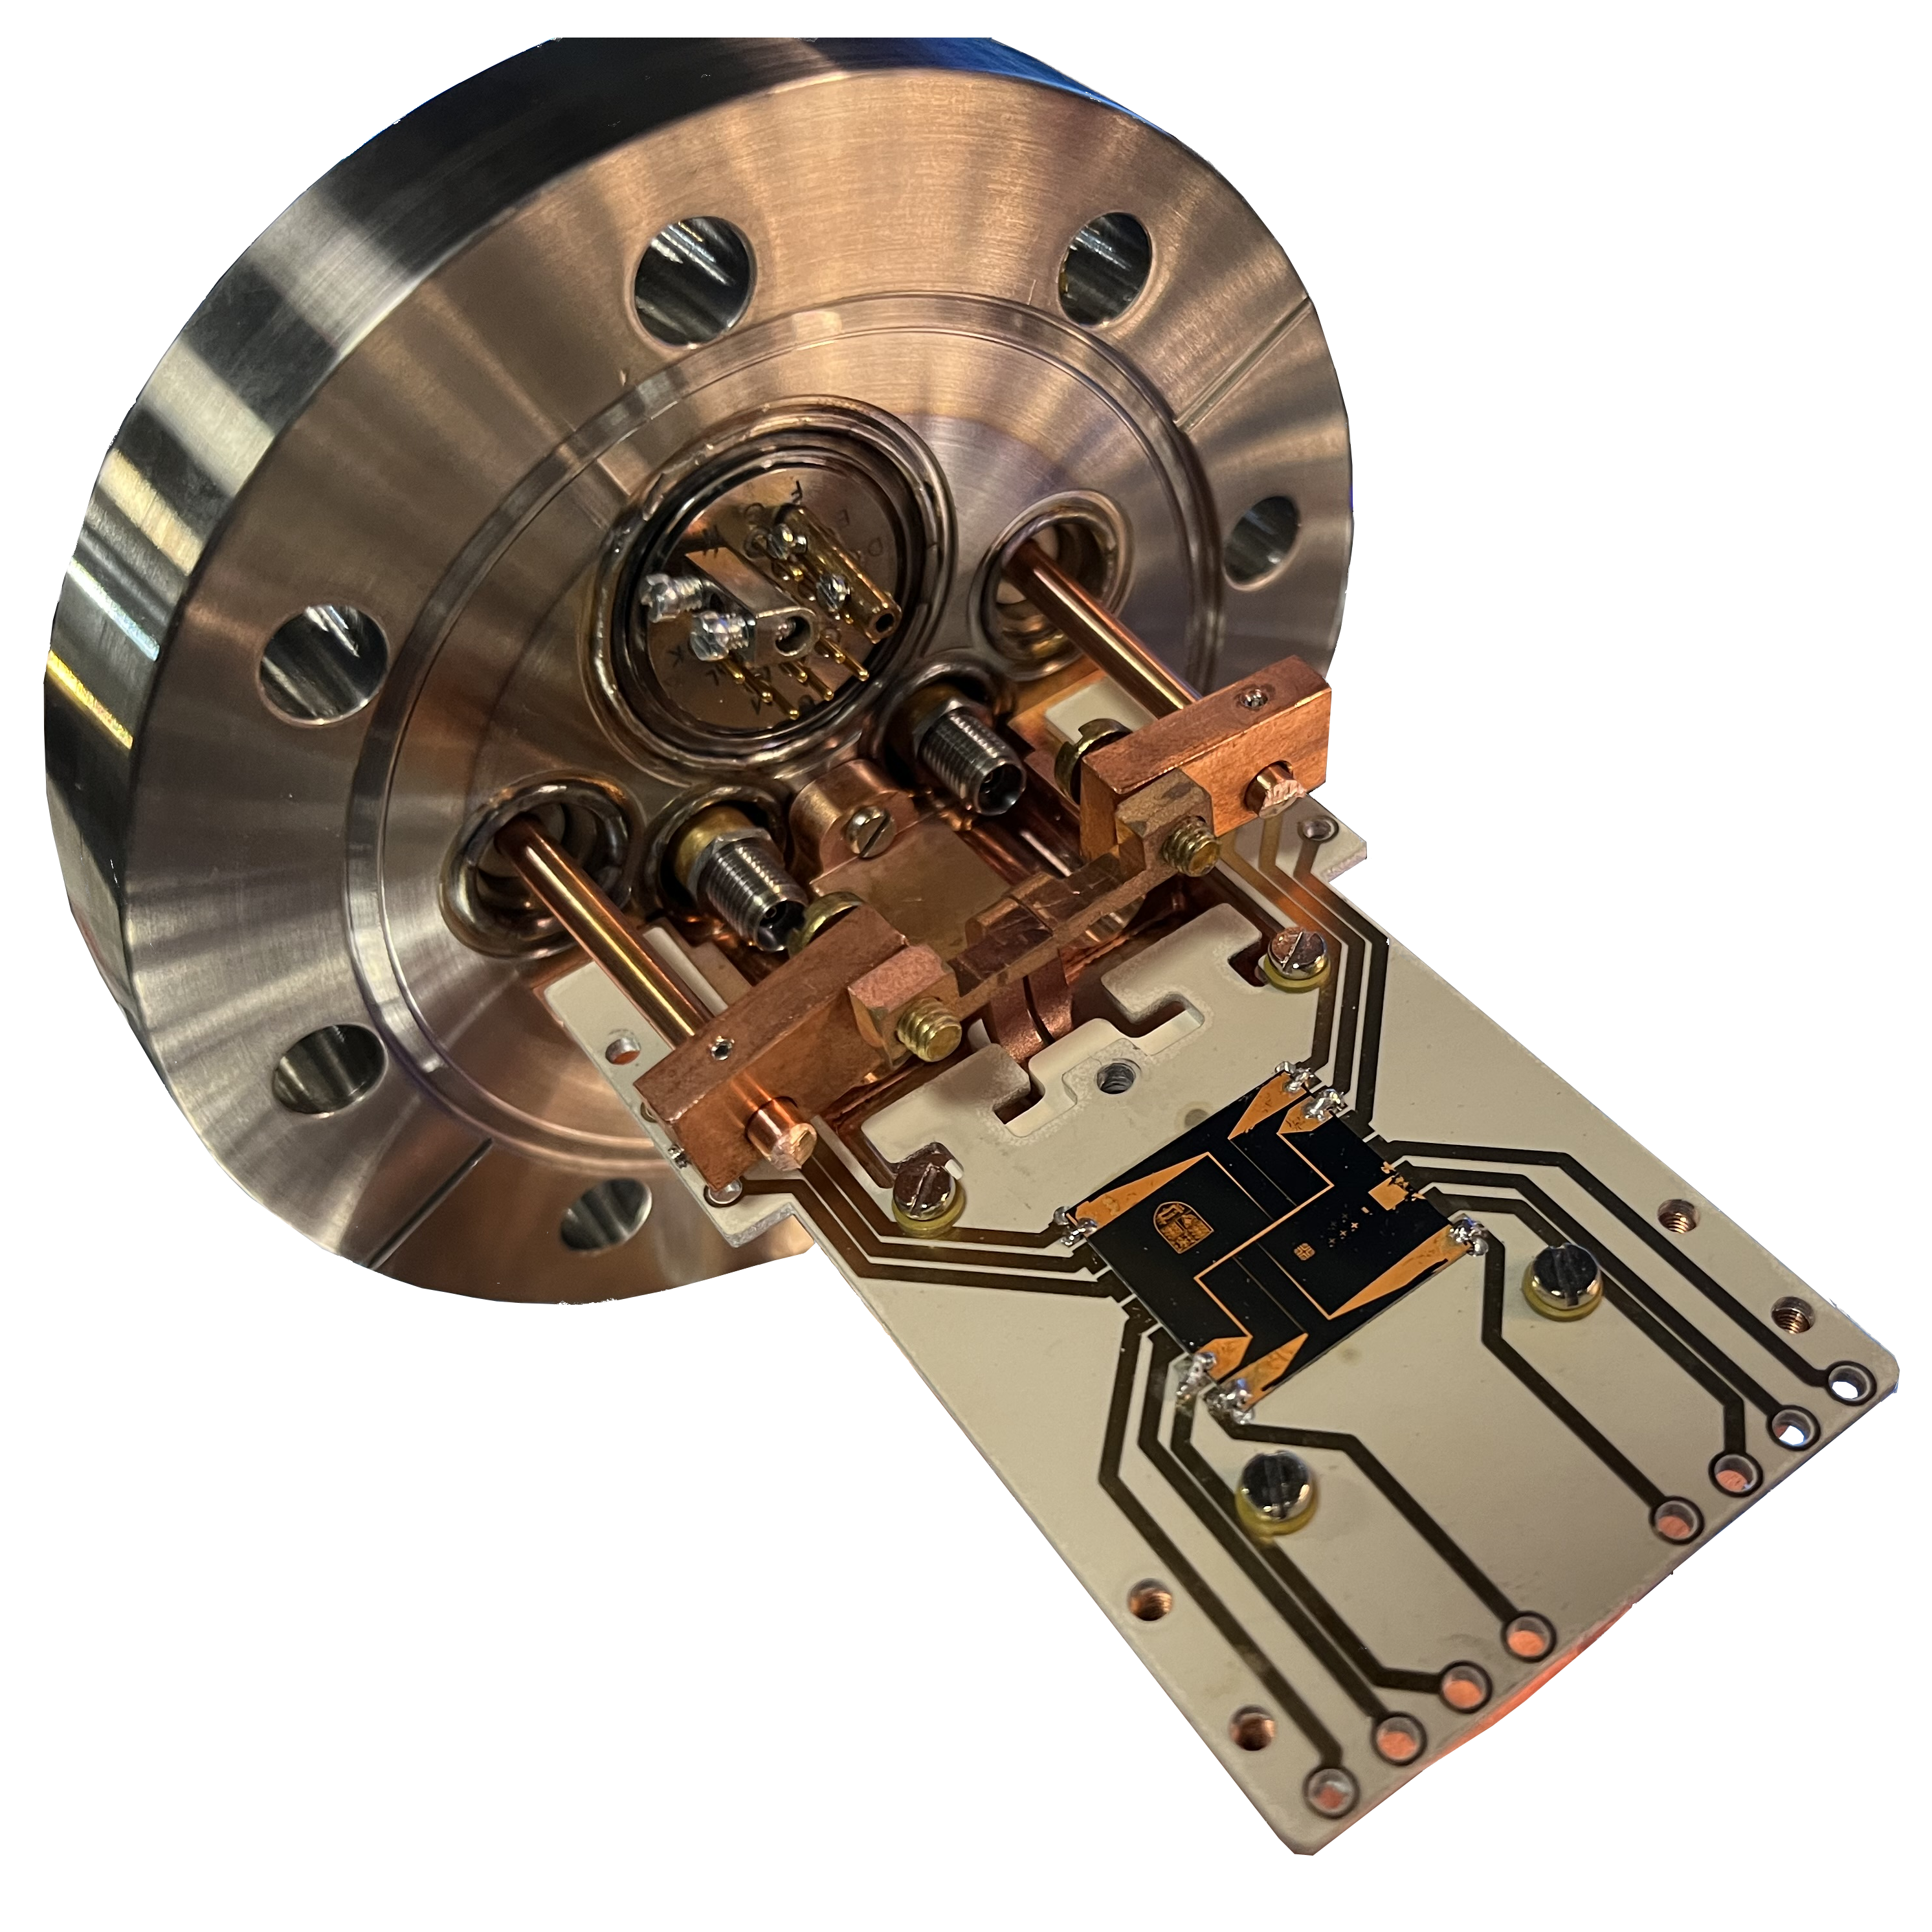
\includegraphics[width=\textwidth]{figs/chip_pic_crop.png}
    \caption{}
  \end{subfigure}
  \hspace{1cm}
  \begin{subfigure}[b]{0.45\textwidth}
    \centering
    \includegraphics[width=\textwidth]{figs/chip_present2.pdf}
    \caption{}
  \end{subfigure}
  \caption{
    In (a) we have the chip assembly fully constructed, with a view of the
    aluminium-core PCB (subchip) for current delivery. Note also the polyimide
    bushings to electrically isolate the retaining screws from the surface. The
    microwave feedthrougs remain disconnected. In (b) we show a schematic of
    the chip features, with the scaling exaggerated for visibility. The three
    overlapping Z-wires are shown. Toward the left is the electroplating
    connection pad and various features used for characterisation, andn the small
  wire there are several anchors to improve adhesion. All of these will be
  discuseed further in chapter~\ref{fab}. The crest of Imperial College London
is also included.}
  \label{design:fig:chipexperiment}
\end{figure}

Since the molecules will be brought into the chamber inside  amagnetic trap,
the natural thing to do seems to be to continue to trap magnetically as we
transfer them onto the chip. Not only does this take advantage of the known,
long-lived \CaF{} states in the trap~\cite{Williams2018}, but it allows us to
follow the well-trodden path of magnetic trapping near a chip, as has been
outlined in previous chapters.  The transfer to the chip will take the
molecules through a series of magnetic traps of decreasing size until they are
in the smallest trap. The design of these traps and the loading
procedure are the main subjects of this chapter.

The first stage of the transfer is a large U wire embedded in the heatsink (see
inset of \myfigref{design:fig:chipexperiment}).  The idea is to use this as a
deep, macroscopic trap that is well-aligned with the chip (by virtue of being
built into the assembly) and can be easily aligned with the MTT, similarly to
other experiments such as \inlineref{Ott2001}.  Since it is under the chip, it
will of course be further from the molecule cloud than the other wires, hence
more current will be required to create a deep trap (as per
equations~\ref{intro:eq:trapbias} and~\ref{intro:eq:trapdepth}). The current is
limited to \SI{100}{\ampere} by the vacuum feedthroughs, allowing for a trap of
depth around \SI{2}{\milli\kelvin} by equation \cm{ref. earlier chapter}.

Once loaded into the U-trap, the molecules will be transferred through the
Z-wire traps on the chip. The idea is that each Z-wire should be sufficiently
large to maintain the currents required to form a trap at height $z$ below the
trap, whilst having a width and height  $w, h \ll z$ so that that the current
is highly localised compared to the cloud size.  This follows the widely-made
assupmption in the literature that the trapping currents are carried by wires
which are infinitesimally small compared to the length scale of the trap
~\cite{2011Ac}.

In the case of the first Z-wire, the molecules are still \SI{4}{\milli\meter}
away from the trapping wire. If we (pessimistically) expect the cloud to have a
temperate on the order of \SI{1}{\milli\kelvin}, then we will require a
trapping current of \SI{30}{\ampere} to form a trap of this depth.  We will
discuss in chapter~\ref{fab} that the maximum wire height achievable is
\SI{5}{\micro\meter}, and we expect that the wires will be able to carry a
maximum current density of \SI{6E10}{\ampere\per\meter\squared}, as was found
for a similar chip design in \inlineref{Treutlein2008}. The Z wire will
therefore have a width $w=\SI{200}{\micro\meter}$. Other wire parameters are
shown in \mytableref{design:table:wires}.

The axial length of the wires also decreases to gradually reduce the size of
the trapped cloud in the $x$ direction. An exaggerated schematic of the wire
layout is shown in \myfigref{design:fig:chipexperiment} and further details are
outlined in \mytableref{design:table:wires}. All wires have been designed to
carry twice the current that is required in the loading scheme.

% TODO Maybe need more detail here
\begin{table}
  \centering
\begin{tabular}{lrrrrr}
  Name & Axis length (\si{\milli\meter}) & Width (\si{\micro\meter})& $I_\text{max}$ & Trap height (\si{\micro\meter}) \\
 \hline
  U & 16 & N/A& 100 & 3000\\
  $\mathrm{Z0}$ & 12 & 200& 60& $3000\rightarrow1000$ \\
  $\mathrm{Z1}$ &  6 & 20& 6& $1000\rightarrow100$ \\
  $\mathrm{Z2}$ &  2 & 2& 0.6& $100\rightarrow10$ \\
 \hline
\end{tabular}
  \caption{Details on the wire dimensions, maximum current, and desired
  trapping heights. The wire design is shown in
  \mysubfigref{design:fig:chipexperiment}{c}. Note that the U wire current is
  limited by vacuum feedthroughs and not by the maximum current calculated by
  the wire dimensions.  The maximum currents have been designed for use at only
  50\% of their potential maximum ($I_\text{max}$).
  }
  \label{design:table:wires}
\end{table}

Each Z trap will begin trapping at one height before the bias field is
increased to bring the trap centre closer to the surface (as per
\myeqref{intro:eq:trapbias}).  To distinguish between the two trap stages for
each wire, we label them $\mathrm{ZX_i}$ for the initial (higher) trap and
$\mathrm{ZX_f}$ for the final (lower) trap, with $\mathrm{ZX}$ corresponding to
the wire labels in \mytableref{design:table:wires}.

A future goal of the project is to incorporate microwave guides onto the chip. This can be
accomplished by adding an insulating layer on top of the wires, on to which we
can fabricate coplanar waveguides~\cite{1127105}. The flange has been designed
with microwave feedthroughs, so that microwaves can be launched onto the
subchip and carried to the chip via coplanar waveguides \cm{to be discussed in
a later chapter}.

Having broadly outlined the experiment, the rest of this chapter will justify
the design of the trapping wires by means of simulation and analysis
of the trapping potentials.

\section{Motion of molecules in a trap}
\label{design:motion}

% TODO Is the Bohr magneton introduced above?
% TODO Do I introduce this ket notation above?
We can assume that the motion of the molecules in the trap is classical. They
move in the potential $V(t, \mathbf{q}) = \mu B(t, \mathbf{q})$, where
$\mu\approx\mu_B$ is the magnetic dipole moment of the molecule in the
$\ket{1,0,-1}$ state.  The motion of any one particle is described by Hamilton's
equations,~\cite{Lichtenberg1969}
%
\begin{align}
  \label{design:eq:hamilton}
  \dot{\mathbf{q}} =  \frac{\partial H}{\partial \mathbf{p}} &&
  \dot{\mathbf{p}} = -\frac{\partial H}{\partial \mathbf{q}},
\end{align}
%
where $H$ is the classical Hamiltonian of the system
\begin{equation}
  %
  H(t, \mathbf{q}, \mathbf{p}) = \frac{\mathbf{p}^2}{2m} + V(t, \mathbf{q}).
\end{equation}
For now we neglect the time dependence of the potential, so that $V(t,
\mathbf{q}) = V(\mathbf{q})$.

Solving Hamilton's equations tells us the position and momentum of a single
particle. Taken together, these two vectors describe a point in a six
dimensional phase-space of position and momentum. The ensemble of
trapped molecules, each one starting at a different point in phase-space, can
be treated by considering the motion of the molecules at its
boundary, and the six-dimensional phase-space volume that this
boundary encloses~\cite{Hand1998}.

It is helpful for us to write the phase-space volume $V$ in terms of the
spatial volume occupied by the ensemble ($V_\text{space}$) and its temperature.
The length-scale for a monatomic gas of temperature $T$ is the thermal de
Broglie wavelength~\cite{blundell2}
%
\begin{equation}
  \lambda_\text{dB}(T) = \frac{h}{\sqrt{2 \pi m k_B T}}.
\end{equation}
%
Hence the unitless phase-space volume is
%
\begin{equation}
  V = V_\text{space} \lambda_\text{dB}^{-3}(T).
\end{equation}
%
It is also useful to define a unitless phase-space
density~\cite{PhysRevA.52.1423}
%
\begin{equation}
  \rho = \frac{N}{V} = \frac{N \lambda_\text{dB}^3}{V_\text{space}}.
\end{equation}
%
For a given cloud with phase-space density $\rho$, trap with volume
$V_\text{trap}$ and depth $T_\text{depth}$,
the maximum possible number of particles that can be trapped is $\rho
V_\text{trap}/\lambda_\text{dB}^3(T_\text{depth})$.

Furthermore, Liouville's theorem~\cite{Landau1982, Hand1998} states that the
phase-space volume is a conserved quantity, as long as the trapping potential
is consevative. This means that the phase-space density of a trapped molecular
cloud cannot be increased without application of some velocity-dependent
damping, such as an optical molasses~\cite{Metcalf1999}. The impact of this for
the chip is that the phase-space density of the cloud at the point of loading
onto the chip determines the maximum number of molecules that can be trapped in
the final trap.

If we do not introduce any further cooling steps, then the number of molecules
we are able to trap in the final trap will be
%
\begin{equation}
  N_\text{final} = \frac{\rho_\text{\CaF{}}V_\text{trap}}
  {\lambda_\text{trap}^3} = \frac{\rho_\text{\CaF{}} V_\text{trap}(2 \pi m_\text{CaF} k_B
  T_\text{trap})^\frac{3}{2}}{h^3}
  \label{design:eq:psd_N}
\end{equation}
%
where $\rho_\text{\CaF{}} = 3.4\times10^{-12}$ is the phase-space density of
the \CaF{} cloud after cooling in the blue-detuned molasses~\cite{Truppe2017},
$V_\text{trap}\sim(\SI{10}{\micro\meter})^3$ and
$T_\text{trap}=\SI{4}{\kelvin}$. The \CaF{} mass is
$m_\text{\CaF{}}=\SI{9.79E-26}{\kilogram}$. The trap depth used here is for the
smallest trap operating at \SI{3}{\ampere}, and can be calculated using
equation~\ref{intro:eq:trapdepth}. We therefore have
%
\begin{equation}
  N_\text{final} \lesssim 2000
\end{equation}
%
as an upper bound for the number of molecules trapped in the final trap. To
reiterate, this assumes that the entire trap is full, and no excess molecules
have been lost during loading. We will see below that this will not be the
case. A more realistic number of molecules to be trapped can be found by using
two key tools: analysis of the phase-space acceptance of the traps, and direct
trajectory simulation of the cloud.

\subsection{Phase-space acceptance}

\cm{Probably need to cite Hand 1998}

For a particle to be trapped, it is obvious that it must exist within the
spatial region of the trap, and it must not have sufficient energy to escape
from the trap's potential. In other words, the Hamiltonian of the particle
$H(\mathbf{q}, \mathbf{p})$ must be less than the trap depth $T_\text{depth}$.
This relation defines a region of phase-space that we call the
acceptance. Any particles within this region will not have sufficient
energy to escape, and so will remain trapped under classical motion unless
externally influenced (ignoring for example any collisions, decays, Majorana
losses, etc.)~\cite{Lichtenberg1969}.

As an example consdier the one-dimensional case of a harmonic trap found in 
\inlineref{Crompvoets2005}
%
\begin{equation}
  V(z) = \begin{cases}
    0 & |z| > l \\
    -\frac{1}{2}m\omega^2 z^2 & |z| \leq l.
  \end{cases}
\end{equation}
%
Here, any particle which starts with a position $l \leq z \leq l$ will be
trapped, so long as its velocity is not sufficiently large that it will escape
into the $|z|> l$ region. To reach $z=l$ from an initial position $z_0$, the
particle must have kinetic energy of at least
%
\begin{equation}
  \frac{1}{2}mv_0^2 = \frac{1}{2}m\omega^2(l^2 - z_0^2)
\end{equation}
%
where $v_0$ is the initial velocity. It is now clear that a particle is trapped
on the condition that
%
\begin{equation}
  (v_0/\omega)^2 + x_0^2 < l^2
\end{equation}
%
which defines an ellipse in phase-space.

% Note that in the simulation I have omega = 1, so taking omeaga -> 1000 means
% that we end up with the nice circle with v in m/s. The consequence is that
% the simulation ends up lasting 1.2ms rather than 1.2s

This trapping region is can be verified by simulation, as is shown in
\mysubfigref{design:fig:psaeg}{a}, where the trap has been simulated for $m =
1$, $\omega = \SI[parse-numbers=false]{10^3}{\radian\per\second}$ and $l
=\SI{1}{\milli\meter}$. We initialise 2000 particles uniformly distributed with
$|z_0| < \SI{0.2}{\milli\meter}$ and $|v_0|< \SI{1.5}{\meter\per\second}$,
their trajectories are computed for \SI{1.2}{\milli\second} by the methods
described in the next section. The boundary of the acceptance, called the
separatrix is shown in black. All particles that are intialised inside the
acceptance remain trapped and evolve through time in the usual way for a
harmonic potential.  Particles initialised outside the acceptance are rejected
and lost.

It is also instructive to consider anharmonic potentials, for example
%
\begin{equation}
  V(x) = -V_0\cos(\omega z)
\end{equation}
%
which is also presented in \myfigref{design:fig:psaeg}, using the same
parameters as for the previous potential. We again see that particles with
sufficiently low energy in the trapping region remain trapped, however in this
case the anharmonicity of the trap results in the particle cloud spiralling
outwards, undergoing an effective increase in the phase-space density.

Finally, it is useful to consider the phase-space acceptance of a wire trap.
For simplicity we begin by considering only the acceptance in the $z$ direction
(perpendicular to the chip surface). Acceptance of a Z-wire with an axis of
\SI{20}{\milli\meter}, current of \SI{40}{\ampere} and a trapping height of
\SI{3}{\milli\meter}. The particles are initialised such that they have no
motion in the $x$ and $y$ directions, and the trajectories are simulated for
\SI{200}{\milli\second}. The distributions as initialised and at the end of the
simulations are shown in \myfigref{design:fig:psaeg}. The accepted
molecules (blue) are once again those that start inside the sepatrix. There are
also metastable molecules (orange) which remain outside the acceptance but stay
nearby the trap. These are molecules with nearly sufficient energy to escape
the trap, but may take some time to do so.

% TODO This caption
\begin{figure}[htb]
  \centering
  \import{figs/simsThesis/}{psa_1D.pgf}
  \caption{
    The phase-space acceptance for harmonic (a, d), anharmonic (b, e) and
    Z-wire trap (c, e) are shown. The top row shows the initial positions of
    the particles, those that are accepted by the trap are shaded blue,
    particles that are lost are shaded red, and metastable particles in orange.
    The energy contour of the trap depth is also shown. The end state of the
    simulation is shown in the lower row. Note the filamentation effect in (e)
    and (f), where the effective phase-space density of the particles increases
    as they explore regions that are energetically accessible. The harmonic and
    anharmonic examples are inspired by discussion in
    \inlineref{Crompvoets2005}.
  }
  \label{design:fig:psaeg}
\end{figure}

It is therefore clear that a particle that is stored in one trap can be moved
into another if its position in phase space is inside the sepatrix of the new
trap. It is therefore in our interest to design the trapping potentials such
that the emission of one trap overlaps with the acceptance of the next one in
the loading sequence. This is similar to the mode-matching of potentials
described in, for example, \inlineref{2011Ac}. We will see below that the
matching of trap acceptances does indeed allow for reliable loading of the
traps

An adiabatic change to the potential will not affect the phase-space density of
any particles that remain trapped throughout the change~\cite{Hand1998,
Lichtenberg1969}. Hence a cloud of trapped particles can be translated, for
example in the transport coils, or towards the surface of the chip as will be
discussed in section~\ref{design:sim}.

It should be noted that the Liouville theorem also holds for a time-dependent
Hamiltonian. We will see below that the trapping potential will be changed
adiabatically, and make use of the fact that phase-space density is conserved
through this process.

\subsection{Simulating the motion}
\label{design:motion:simmethods}

The motion of a particle can be simulated by numerically solving
\myeqref{design:eq:hamilton}, which we do using Python~\cite{python} and the
symplectic Euler method~\cite{Hairer2015, doi:10.1119/1.2034523} provided by
the Desolver package~\cite{desolver}.  Symplectic methods are powerful tools
for numerically solving Hamiltonian systems whilst conserving energy and
momentum.

We are able to simulate any arbitrary potential, such as those already
discussed in the previous section, but it is useful to consider a more
realistic potential given by the sum of the magnetic and gravitational
potentials,
%
\begin{equation}
  V(t, \mathbf{q}) = V_\text{mag} + mg(z_0-z)
\end{equation}
where $g=\SI{9.8}{\meter\per\second\squared}$ is the acceleration due to
gravity, and $z_0$ is an arbitrary point chosen to be the zero of the
gravitational potential. The actual value chosen does not matter as it
constitutes only a linear shift in the entire potential, we normally present
the potentials with $z_0$ chosen such that the trap minimum is zero.

The Van der Waals attraction between the chip and the molecules is neglected,
since the molecules will (by design) never be close enough to the chip for this
force to be significant.

When simulating the motion of the particles in a quadrupole coil trap (such as
the MTT), the magnetic field is assumed to be an idea quadrupole, so
%
\begin{equation}
  \mathbf{B}(x, y, z) = B'\begin{pmatrix} -x/2 \\ -y/2 \\ z \end{pmatrix}
\end{equation}
where $B'$ is the field gradient.

The magnetic potentials of the wire traps are calculated by considering the
traps to be formed of segments of straight wires, each producing a magnetic
field $\mathbf{B}_\text{seg}^{(i)}$, and the bias field
$\mathbf{B}_\text{bias}(t)$.  The total field is the sum of contributions from
the set of all segments (S), and the bias. The potential is therefore
%
\begin{equation} V\text{mag}(t, \mathbf{q}) = \mu B (t, \mathbf{q}) = \mu
\left| \sum_{i\in S} \mathbf{B}_\text{seg}^{(i)}(t, \mathbf{q}) +
\mathbf{B}_\text{bias}(t)\right|.  \end{equation}
%
Where the field of each wire segment is~\cite{Griffiths2017}
%
\begin{equation} \mathbf{B}_\text{seg}(t, \mathbf{q}) = \frac{\mu_0 I(t)}{4\pi
s_\text{seg}(\mathbf{q})} (\sin(\theta_2)  -
\sin(\theta_1))\hat{\mathbf{\phi}}. \label{design:eq:segmentfield}
\end{equation}
%
Here $s_\text{seg}(\mathbf{q})$ represents the shortest distance between the
point $\mathbf{q}$ and the line that runs through the segment off to infinity
in each direction. We also have the unit vector $\hat{\mathbf{\phi}} =
\mathbf{I}\times\mathbf{q}/(qI)$.

\begin{figure}[h]
\centering
  \begin{tikzpicture}
    % Def coords
    \coordinate (O) at (0, 0);
    \coordinate (L) at (-3, 0);
    \coordinate (R) at (3, 0);
    \coordinate (Q) at (-4, 4);
    % Draw lines
    \draw[line width=0.75mm, ->] (L) -- (R);
    \draw (L) -- (Q);
    \draw (R) -- (Q);
    \draw[<->, densely dotted,shorten >=.5mm,shorten <=.8mm] (Q) -- (-4, 0);
    % Draw line parallel to wire
    \draw[-, dashed] (-5, 0) -- (L);
    \draw[-, dashed] (R) -- (5, 0);
    % Draw dot at Q
    \node at (Q)[circle,fill,inner sep=.5mm]{};
    % Draw angels
    \draw pic[draw,angle radius=1cm,"$\theta_1$" shift={(7mm,2mm)}] {angle=R--L--Q};
    \draw pic[draw,angle radius=1cm,"$\theta_2$" shift={(-7mm,2mm)}] {angle=Q--R--L};
    % Label
    \node[shift={(4mm,0)}] at (Q) {$\mathbf{q}$};
    \node[shift={(2mm, 4mm)}] at (R) {$I$};
    \node[fill=white] at (-5.0, 1.8) {$s_\text{seg}(\mathbf{q})$};
  \end{tikzpicture}
  \caption{Geometry of a wire segment (bold) carrying current $I$, whose field
  can be calculated using \myeqref{design:eq:segmentfield}. The dotted line
  shows $s_\text{seg}(\mathbf{q})$, the shortest distance from the point at
  which the field is calculated ($\mathbf{q}$) to the line parallel with the
  wire (dashed line).
  }
  \label{design:fig:wiresegment}
\end{figure}

In the case of that we are exchanging between
two potentials, the segments of both traps are included in the summation, with
the currents becoming functions of time, and similar for excahnge between a
quadrupole and a wire trap, with the quadrupole gradient being a function of
time.


\subsection{Simulation initialisation}

For all the simulations described below, we begin with a cloud of molecules in
a magnetic quadrupole trap. We use the following initialisation procedure s
that the distribution of our molecules matches that which we expect in the
experiment. 

We begin with a cloud of $N$ molecules whose positions are normally distributed
in all three spatial dimensions with a standard deviation of $\sigma_i$
(typically $\sigma_i = \SI{1}{\milli\meter}$. Similarly the velocity components
are normally distributed with a standard deviation of $\sigma_{v_0}$ (typically
\SI{84}{\milli\meter\per\second}, corresponding to a temperature of
\SI{50}{\micro\kelvin}). 

The cloud is immediately placed in a quadrupole trap with gradient
\SI{10}{\gauss\per\centi\meter}. They are held for \SI{50}{\milli\second}
before the gradient is ramped up over \SI{100}{\milli\second} to the 
\SI{60}{\gauss\per\meter} (the gradient used in the MTT).
The molecules are then held for a further \SI{50}{\milli\second}, as a
stabilisation time.

The increasing trap gradient causes the
molecules to compress as they would when initially loaded into the transport
coils in the MOT chamber, as can be seen in \myfigref{}.
\cm{Need to show histograms in radial and axial, along with comparison to real
data, which I should collect.}

\section{Adiabatic transfer between traps}

% Simple QP ramp (varying time to find adiabatic regime)

In fact, the simple potential of a quadrupole potential can be used to
illustrate a point about transferring molecules between traps. It should be
obvius that if we start with molecules in one potential, then rapidly turn that
one off and turn on another, this will cause heating and increasing its size.
However, if we ramp between the traps adiabatically, then we expect the effect
to the cloud size to be minimal.

In our example, we will consider two ideal quadrupoles with gradients of
\SI{60}{\gauss\per\centi\meter} separated by \SI{3}{\milli\meter} in the $x$
direction. We simulate 2000 \cm{?} molecules using the above-described
initialisation procedure and \cm{sigma and temp values} and ramp between the
potentials in a time $t_\text{ramp}$, which we vary between
\SI{1}{\milli\second} and \SI{100}{\milli\second}. The molecules are then held
for a further \SI{100}{\milli\second}. The state of the system at the end of
the simulation is shown for $t_\text{ramp}\in \{\SI{1}{\milli\second},
\SI{30}{\milli\second}, \SI{100}{\milli\second}\}$ in \cm{figure}, along with
the behaivour of the cloud in the \SI{100}{\milli\second} hold time. Note that
as the ramp time increases, the oscillation in cloud size, temperate and
position decreases, as we have said we expect.

\begin{figure}[p]
\centering
  \import{figs/simsThesis/}{adiabatic_3sim.pgf}
  \caption{
  }
  \label{design:fig:adia3sim}
\end{figure}


The question then is at what point do we enter the adiabatic r\'egime? \cm{Some
figure} shows the cloud width and temperature at the end of the simulation for
varying $t_\text{ramp}$. After $t_\text{ramp}\sim\SI{50}{\milli\second}$ \cm{we
are pretty adiabatic}.

\begin{figure}[tbhp]
\centering
  \import{figs/simsThesis/}{adiabatic_varyramps.pgf}
  \caption{
  }
  \label{design:fig:adiavary}
\end{figure}

\cm{In this figure, note that the rapid oscillations in x width probably
account for the weirdness at the start of the width graph.}

% Z transfer (c.f. rapid)

\section{Trajectory simulation of the initial loading stages}

To ensure that the chip design will allow for robust loading, the loading
process has been simulated up to the $\mathrm{Z0_f}$ trap. This demonstrates
the two main types of transitions in the loading process: handovers between
traps, and compression within a single trap. The timing of the simulation do
not exactly reflect those that will be used in practice, long holding periods
have been inserted between ramps to better illustrate the cause of particle
loss.

The results of the simulation and the parameters of the ramps are outlined in
\myfigref{design:fig:simparams}.
%TODO Redo this old nonsense
\cm{This can be considered in four parts, first
from $t = 0$ to $t=\SI{100}{\milli\second}$ there is a settling period where
the molecules are held in the transport trap. Then there are three
\SI{100}{\milli\second} ramps, each of which is followed by a
\SI{100}{\milli\second} stabilisation period. These three ramps describe the
handover from the transport trap to the U, the U to $\mathrm{Z0_i}$, and the
compression of $\mathrm{Z0_i}$ to $\mathrm{Z0_F}$. They are described in detail
in the following subsections. This simulation used $N=1000$ particles, with one
particle lost during initialisation.}
\cm{For this fig. I think I just want all the parameters, temp, ramps,etc in
one go, similar to before.}



\subsection{MTT - U transfer}
\label{design:sim:trans_U}

\begin{figure}[p]
\centering
  \import{figs/simsThesis/}{mtt_u_summary.pgf}
  \caption{
    The particle distribution in the MTT (blue) and after transfer to the U
    trap (red) following the process described in the main text. The
    phase-space distributions are shown in the $z$-$v_z$ plane in (a) and (b),
    with histograms of the $z$ and $v_z$ projections in (c) and (e)
    respectively. The potentials at the start and end of the transfer are shown
    in (d). Subfigure (f) shows the temperature particle number varying
    throughout the fields are varied in the times that are shaded grey (c.f.
    \myfigref{design:fig:simparams}). \cm{Comment on the results.}
  }
  \label{design:fig:mttusum}
\end{figure}




\cm{Ensure language is consistent when talking about chip, so is the U
above or below?}
%
The first step is to transfer the molecules from the transport coils to the U
wire. This U wire has the largest axial length, and so will be the easiest trap
the transport coils to. The U-wire is also capable of carrying more current
than any of the other wires, which is essential as it is positioned further
from the molecule cloud, beneath the chip.

Between $t=\SI{100}{\milli\second}$ and $t=\SI{200}{\milli\second}$ the current
in the transport coils is adiabtically ramped down while the currents in
the U trap and in the bias coils are ramped up. The molecules are then held
until $t=\SI{300}{\milli\second}$ to ensure that they remain trapped after the
ramp. The simulation parameters are shown in
\mysubfigref{design:fig:simparams}{b}.

The particle loss during the ramp is approximately 10\% of the total. There is
also some heating, which decreases the phase-space density of the cloud. The
cause of this can be seen in \myfigref{design:fig:trans_U}, which shows the
phase-space positions of the molecules at various times throughout the ramp,
and the trapping potential at those times.

\begin{figure}[p]
\centering
  \begin{tabular}{c}
  \import{figs/simsThesis/}{mtt_u_detail_x.pgf} \\
  \import{figs/simsThesis/}{mtt_u_detail_y.pgf} \\
  \import{figs/simsThesis/}{mtt_u_detail_z.pgf}
  \end{tabular}
  \caption{
    Each pair of rows shows the phase-space plots for the MTT to U trap
    handover simulation in the $q_i$-$v_i$ plane, along with the cut-through of
    the potential through the trap centre along $q_i$ at various times. This
    supplements the simulation summary shown in \myfigref{design:fig:mttusum}.
    The superposition of the quadrupole and U-traps briefly causes a lowering
    of the trapping potential, as can be seen at \cm{time??} in the $y$
    direction. Such reductions are not accounted for when considering the
    simple phase-space handovers discussed in the main text.
  }
  \label{design:fig:mttudetail}
\end{figure}

At $t=\SI{175}{\milli\second}$ there is a noticeable decrease in the trapping
depth in the $y$ direction. This is the cause of the particle leak, and occurs
due to the due to the superposition of the two fields causing an overall
decrease in the trap depth in the $x$ and $y$ directions. This only occurs for
a brief period during the ramp (lasting approximately \SI{40}{\milli\second}). 

In addition to the loss during the ramp, we observe a steady loss between
$t=\SI{200}{\milli\second}$ and $t=\SI{300}{\milli\second}$, but only when the
simulation accounts for collision with the chip surface. This loss due to
collision occurs in the U wire because of its position beneath the chip. This
means that the trap is not sufficiently deep to hold our molecules for an
extended period. However the holding time in this simulation is only for
illustration, and the prolonged trapping in the U trap will not be part of the
final experiment. Hence these losses can be ignored.

\subsection{U - Z transfer}
\label{design:sim:U_to_Z0i}

\begin{figure}[p]
\centering
  \import{figs/simsThesis/}{u_z_summary.pgf}
  \caption{
    The U trap to Z trap handover is summarised, with subfigures and colours as
    in \mysubfigref{design:fig:mttusum}. Here we again see loss effects similar
    to those seen for the MTT to U trap handover, with a decrease in trap depth
    \cm{that may be} due to changing from a quadrupole trap to a
    Ioffe-Pritchard trap.
  }
  \label{design:fig:uzsum}
\end{figure}

The U to $\mathrm{Z0_i}$ handover occurs in our simulation from
$t=\SI{300}{\milli\second}$ to $t=\SI{400}{\milli\second}$, shown in
\mysubfigref{design:fig:simparams}{c}.  The phase-space positions of the
molecules and the potentials are shown in \myfigref{design:fig:U_Z0i}.

In the ramp between the transport trap and the U trap, we saw that a hole was
introduced in the trapping potential due to interference between the two
trapping fields. We will see a similar effect when transferring from the U trap
to trap $\mathrm{Z0_i}$.  This time the reduction in depth appears in the $x$
direction, and is due to the current in the U and Z wires opposing each other
on the positive $x$ side. This can be seen in \myfigref{design:fig:U_Z0i} at
$t=\SI{375}{\milli\second}$.

In \myfigref{design:fig:simparams} we see that the loss is again about 10\% of
the particles, however there is no significant change in the phase-space
density. The acceptance of trap $\mathrm{Z0_i}$ is smaller than the emittance
of the U, so this is to be expected.

\subsection{Z compression}
\begin{figure}[p]
\centering
  \import{figs/simsThesis/}{z_summary.pgf}
  \caption{
  }
  \label{design:fig:mttusum}
\end{figure}


In the final stage of the simulation we look at a compression stage. The
trapping potential is adiabatically altered to bring the field minimum closer
to the chip surface. This is achieved by increasing the bias field, but since
this also increases the trap depth the cloud is simultaneously compressed as it
is heated. Since the phase-space density is conserved, the particles heat up in
the trap. This phenomenon is made visible in
\mysubfigref{design:fig:simparams}{d}.

The trajectories and potentials are shown in \myfigref{design:fig:Z0i_Z0f}.
Here the compression in number density and expansion in velocity space is clear
by the changing cloud shape over time. The cloud also clearly follows the
potential minimum without losses.

\begin{figure}[p]
\centering
  \import{figs/simsThesis/}{total_summary.pgf}
  \caption{
  }
  \label{design:fig:mttusum}
\end{figure}


\section{Phase-space acceptance of remaining Z traps}
\label{design:transferbetweenzs}

\cm{Revisit this spiel.}

Once trapped in $\mathrm{Z0_f}$, the remaining loading stages are simply
repeated handovers to the smaller wires, with a compression stage carried out
on each wire to bring the molecules closer to the surface. This is a
well-understood and robust procedure that has been used before to load atom
chips with minimal losses~\cite{Reichel2002}.

That said, since our experiment will operate with a significantly lower phase
space density than previous experiments with atoms, it is important to ensure
that our loading procedure will not suffer from any unnecessary losses. These
compressed traps contain hotter molecules, requiring a smaller time step for
simulation. It is therefore easier to directly examine the acceptance of each
trap.

These are shown in \myfigref{design:fig:phasematchinggrid}, starting with
$\mathrm{Z0_f}$ in row (a). The region of the trap that we expect to be
occupied (as determined by the simulation above) is marked with a dashed line.
This cloud of molecules will be adiabatically transferred into $\mathrm{Z1_i}$.

Since the process is adiabatic, we can anticipate that there will be no
reduction in phase-space density. The cloud of molecules will be transferred to
$\mathrm{Z1_i}$ with negligible heating. However, the total acceptance of the
trap is less than the expected phase-space volume of the cloud, so there
will be particle loss due to spillover.

This was anticipated in section~\ref{design:motion}: phase-space density cannot
increase in a conservative potential, and the acceptance of the smallest trap
will be smaller than the initial cloud in the transport trap. So the final
number of particles will be lower than we started with, as calculated in
\myeqref{design:eq:psd_N}.

Next, $\mathrm{Z1_i}$ is adiabatically compressed to $\mathrm{Z1_f}$, with the
molecules held \SI{100}{\micro\meter} from the surface. Again, this
compression is adiabatic, so we expect no change in the phase-space density.
Compression increases the trap acceptance, so there is also no loss of
particles. This is further supported by the simulated compression of
$\mathrm{Z0_i}$ to $\mathrm{Z0_f}$ discussed above. The acceptance of
$\mathrm{Z1_I}$ is shown in \mysubfigref{design:fig:phasematchinggrid}{b}, with
the expected occupation shown by the dashed line.

Finally, $\mathrm{Z2}$ is loaded and compressed in exactly the same way as
$\mathrm{Z1}$. The adiabatic handover from $\mathrm{Z1_f}$ to $\mathrm{Z2_i}$
is the final cause of particle loss (due to spillover). Then the trap is
compressed to hold the particles \SI{10}{\micro\meter} from the surface, as
shown in \mysubfigref{design:fig:phasematchinggrid}{c}.


\begin{figure}[htb]
\centering
  \begin{overpic}[page=1]{figs/sims/phase_matching_grid.pdf}
    \put(0,68){(a)}
    \put(0,44.5){(b)}
    \put(0,21){(c)}
  \end{overpic}
  \caption{
    A low bound of the acceptance (solid) and expected occupation (dashed) of
    each Z wire trap. This is calculated by finding the acceptance in the weak
    ($x$) trapping direction. Row (a) shows $\mathrm{Z0_f}$, with occupation
    determined by the above simulation. Molecules will be adiabatically
    transferred to $\mathrm{Z1_i}$, which will be fully occupied. Some
    particles will be lost due to the decrease in acceptance but this is to be
    expected, and phase-space density should not increase. In (b) we have the
    acceptance and occupation of $\mathrm{Z1_f}$ following adiabatic
    compression.  Particles will be adiabatically transferred into
    $\mathrm{Z2_i}$, resulting in similar losses to the previous step.  Row (c)
    shows the final acceptance and occupation of $\mathrm{Z2_f}$.
  }
  \label{design:fig:phasematchinggrid}
\end{figure}


\section{Summary}

In this chapter I have presented the design of the chip experiment, starting
with the source of molecules up to the stage of confinement in a Z trap
\SI{10}{\micro\meter} from the chip surface. I have shown that we have created
a loading procedure that will allow us to load this final trap through a series
of wire traps of decreasing size. This is justified by simulation and visual
analysis of the acceptance of the various trapping stages.

The design leaves scope for the addition of microwave guides on a second layer
above the trapping wires, as discussed in chapter~\ref{intro}.


\chapter{Microfabrication}
\label{fab}
Fabrication of a chip has been an iterative process, where we have
simultaneously improved upon both the chip's design and our fabrication
techniques.
In this chapter I will present the progress that we have made in
learning how to build a chip trap, and how we plan to integrate a microwave
guide in future experiments. 

All the microfabrication techniques described below except for the
electroplating were undertaken at the London Centre for Nanotechnology (LCN). 

\section{Overview of the fabrication procedure}

% TODO I grabbed this Madou2002 citation from Treutlein, but I should ensure
% that it is legit
Our trap has been designed so that the size of the wires is small compared to
the size and height of the trapped cloud. As such trapping wires on the chip
are as small as \SI{3}{\micro\meter} in width. Such small features can be
produced using standard photolithography techniques~\cite{Madou2002}. However,
the maximum height of features produced in these procedures is usually of the
order \SI{100}{\nano\meter}.

% TODO Need to cite this $j$ number
We must ensure that the wires are capable of carrying the currents that are
outlined in chapter~\ref{design}.  Other experiments with two-layer atom chips
have reported a current density of $j=\SI{6E10}{\ampere\per\meter\squared}$ in
the trapping wires. For our wires this would require a minimum height of $h
\sim I w/j = \SI{1}{\ampere} \times
\SI{10}{\micro\meter}/\SI{6E10}{\ampere\per\meter\squared} \sim
\SI{1}{\micro\meter}$  to carry our trapping currents.This is much higher than
can be achieved with photolithography techniques.

To achieve the required height, we have used through-mask
electroplating~\cite{Ruythooren_2000}. First a substate is coated with a thin
seed layer of gold, then photolithography is used to produce a thick (several
mircron high) mould. The mould covers regions where no further deposition is
required. The substrate can then be electroplated, with the seed layer acting
as the anode, allowing thick wires to be deposited into the mould.
After electroplating the seed layer can be etched away. This is a common
technique for constructing atom chips and is described in \inlinerefs{2011Ac,
Lev2003, KOUKHARENKO2004600}.

The fabrication process for our final chip begins with a four inch silicon
wafer, which we dice into individual \SI{20}{\milli\meter} by
\SI{20}{\milli\meter} dies. The remaining process can be briefly summarised:
\cm{Is there a better way to link this list to the following sections?}
\begin{enumerate}
\item Lay down thin (\SI{60}{\nano\meter}) seed layer of chromium and gold.
\item Spin coat a thick (\SI{6}{\micro\meter}) layer of photoresist.
\item Expose and develop the thick photoresist so as to create a ``mould''
in the desired shape of the wires.
\item Electroplate the chip, such that wires are formed in the mould to the
desired height.
\item Remove the photoresist mould.
\item Chemically etch the chip so as to remove the seed layer and
  electrically isolate the wires.
\end{enumerate}
This process is illustrated in \myfigref{fab:fig:process}

\begin{figure}[h]
\vspace{0.8cm}
\centering
\begin{tabular}{cccc}
  %\begin{overpic}[width=0.22\textwidth]{figs/fab/cartoon/01_barewafer.pdf}
  %  \put(0,40){(a)}
  %\end{overpic} &
  \begin{overpic}[width=0.22\textwidth]{figs/fab/cartoon/03_wafercrauwarrows.pdf}
    \put(0,40){(1)}
  \end{overpic} &
  \begin{overpic}[width=0.22\textwidth]{figs/fab/cartoon/03.5_waferpr.pdf}
    \put(0,40){(2)}
  \end{overpic} &
  \begin{overpic}[width=0.22\textwidth]{figs/fab/cartoon/04_wafermould.pdf}
    \put(0,40){(3)}
  \end{overpic} \\[2cm]
  \begin{overpic}[width=0.22\textwidth]{figs/fab/cartoon/e.pdf}
    \put(0,40){(4)}
  \end{overpic} &
  \begin{overpic}[width=0.22\textwidth]{figs/fab/cartoon/f.pdf}
    \put(0,40){(5)}
  \end{overpic} &
  %\begin{overpic}[width=0.22\textwidth]{figs/fab/cartoon/g.pdf}
  %  \put(0,40){(g)}
  %\end{overpic} &
  \begin{overpic}[width=0.22\textwidth]{figs/fab/cartoon/h.pdf}
    \put(0,40){(6)}
  \end{overpic}
\end{tabular}
  \caption{
    Illustration of the fabrication process. We begin with in (1) with a
    silicon die (black), on which we deposit chromium adhesion layer (grey) and
    a seed layer of gold (yellow). In (2) the entire die is spin coated in
    photoresist (purple). The mould is formed by photolithography techniques
    (3) and then electroplating is used to form tall wires (4). The photoresist
    is removed (5), and then a gold etch followed by a chrome etch (6) are used
    to electronically isolate the features.
  }
  \label{fab:fig:process}
\end{figure}

As discussed in chapter~\ref{intro}, a future aim of the molecule chip project is to
integrate microwave guides on the chip. These guides must allow good overlap of
the microwave fields and the molecule trapping region. Our design achieves this
by positioning the microwave guides on a second layer, directly above the
trapping wires. We have not yet attempted the following stages of
fabrication, but we anticipate that they will be:
\begin{enumerate}[resume]
    \item Spin coat chip with an insulating layer of polyimide.
    \item Perform standard photolithography to lay down microwave guides on the
      chip.
\end{enumerate}
These steps are discussed further in section~\ref{fab:planned}.

In the rest of this chapter I will describe the above process in detail,
including the various pitfalls that we found as we itterated towards a complete
\cm{trapping chip}.

\section{Metal evaporation of seed layer}

Before any fabrication, the die must be cleaned and dehydrated to ensure that
there will be good adhesion to the substrate. A solvent clean with acetone and
isopropyl alchol will remove any organic compounds \cm{check this}. The die is
then rinsed with deionised water and dehydrated in an oxygen plasma for ten
minutes.

The die is then ready for metalization, which here is done by metal
evaporation. To further improve adhesion between the gold and silicon, a thin
($<10\si{\micro\meter}$) intermediary chrome layer is deposited first, followed
by \SI{50}{\micro\meter} of gold.

We performed evaporation using an Edwards A306 bell jar evaporator. Typically
we \cm{metalize} four dies at a time. They are loaded into the belljar, along
with gold and chrome, using a boat and rod respectively.  we deposit gold onto
four dies at a time. The dies are positioned with the polished side facing down
towards the metal. This arrangement is shown in \myfigref{fab:fig:belljar}.

\begin{figure}
  \centering
  \ph{Photo of bell jar with evaporation and layout cartoon}
  \caption{\ph{caption}}
  \label{fab:fig:belljar}
\end{figure}

The belljar is pumped down to pressures below $10^{-6}\si{\milli\bar}$ over a
few hours. The metal for deposition can be selected from a carousel, and heated
by electric current inducing evaporation.  A shutter is used to block
deposition onto the substrate until the desired current has been reached.

The Edwards bell jar evaporator incorporates a FTM7 deposition monitor, which
reports the rate of deposition and automatically shuts off deposition once the
desired thickness has been reached by closing the shutter. \cm{What
determines/ limits the deposition rates? What happens when we have too much
current?}

The deposition rate of gold is typically \SI{0.2}{\nano\meter\per\second}.
%
\cm{Find a way to cite LCN for this and maybe some other factoids.}
%
As discussed above a thickness of \SI{5}{\micro\meter} is desirable for the
chip's trapping wires. Achieving this with evaporation would take over an hour,
and it would not be possible to load the evaporator with enough gold to last
this long. This is why we must use electroplating to achieve the desired
thickness.

\section{Spin coating of photoresist}
\label{fab:spin}

Spin coating is a procedure for distributing a uniform layer of liquid such as
photoresist  across a substrate~\cite{Cohen2011}. It is typically followed by
baking to solidify the layer. We use spin coating to apply SPR220-7 \cite{}
photoresist, which will form the mould for the wires.

The die is mounted in the \cm{spin coater details}, and \cm{how much? I can
check pippete...} of SPR220-7 is applied. The die undergoes a
\cm{\SI{2}{\second} ramp to \SI{500}{\rpm} where it is held before a ?second
ramp to \SI{4000}{\rpm} and held for \SI{30}{\second}.} This results in a
nominal \SI{6}{\micro\meter} high coating of photoresist \cm{according to LCN,
but we haven't actually varified this}.
SPR220-7 requires a post-application bake, first at \SI{90}{\celsius} for two
minutes, then immediately afterwards at \SI{120}{\celsius}.

Spin coating the photoresist results in a bead at the edge of the die. This
thick region of photoresist may not receive sufficient exposure to fully
develop later. This can cause defects in features near the edge. It is
possible to remove the bead by inserting an intial exposure and development
step before the lithography discussed in the next section. However, since the
only features that are covered by the bead are the robust wire bond pads, this
is deemed unnecessary for our purposes. \cm{Defects due to the presence of a
bead can be seen in \myfigref{}.}

\section{Lithography of the wire mould}

Lithography is the process of projecting the image of a design onto the surface
of the substrate. The usual procedure is to coat the substrate in a
photoresist, which can be exposed to ultraviolet light. In our case, SPR220-7
is a positive photoresist, meaning that exposed regions of the
photoresist can be removed from the wafer by submersion in a suitable
photoresist developer. Here, \cm{find name!} was used. 

The common and, perhaps, traditional way to perform photolithography is to use
a \cm{mercury} lamp and a chrome-on-glass mask to cast light onto the
substrate, with the mask casting a shadow so as to illuminate only the desired
region~\cite{Madou2002}. This was the method that we began using at the start of the
project, however we found that it was easier to achieve reliable results by
using the the Heidlberg DWL 66, a direct writer~\cite{}. 

Instead of using a mask to cast a shadow, the direct writer uses a tightly
focused ultraviolet laser, whose beam is raster scanned across the surface. The
beam is then switched on and off so as to produce the pattern that is required.
This process is depicted for a in \myfigref{fab:fig:methods}. The Heidelberg
DWL 66 is capable of producing features down to \SI{300}{\nano\meter} in size.
For SPR220-7 an exposure energy of \cm{??} is required, which is administered
over three passes of the laser at \cm{intensity}. The whole scan for one die
takes around twenty minutes.

Since designs can be directly uploaded to the direct writer, there is no need
to wait for a third party to construct a mask.  Hence the direct writer allows
rapid prototyping. It also has the benefit of making alignment easier, since
this can be performed automatically by the computer, and any issues with
mask-die contact are avoided entirely.


\begin{figure}[h]
\vspace{0.8cm}
\centering
  \begin{overpic}[width=0.8\textwidth]{figs/fab/cartoon/throughmask.pdf}
    \put(10,-5){(a)}
    \put(35,-5){(b)}
    \put(61,-5){(c)}
    \put(86,-5){(d)}
    \put(-1,6){$h$}
    \put(23.2,-0.4){$x$}
  \end{overpic}
  \vspace{10mm}
  \caption{An illustration of how lithography is used to produce tall wires in
  through-mask electroplating. The top row shows a top-down view of the die,
  with a cross section along the dashed line shown in the middle row. The
  bottom row shows a profile of the target (as discussed in
  section~\ref{fab:inspmould}). Column (a) shows photoresist (purple) above the
  seed layer (\cm{colours as in \myfigref{}}) with the exposed region
  highlighted (light blue). The raster scan of the direct writer laser across
  the substrate is highlighted in the top view.  In column (b) the resist is
  developed and the seed layer is exposed. In column (c) gold is deposited via
  electroplating (as discussed in section~\ref{fab:eplate}) to just below the
  height of the mould. In column (d) the photoresist is removed, leaving the
  tall wires (highlighted with black outline) and seed layers, the latter of
  which will be removed by etching.
  }
  \label{fab:fig:tmep}
\end{figure}


This photoresist requires a rehydration step after exposure, so it is left at
ambient temperature overnight before it is developed with  \cm{what? for how
long?}. \cm{Reference first side-on fig.}


\subsection{Inspecting the photoresist mould}
\label{fab:inspmould}

\cm{Profiling, with examples and contact testing of the wire bond pads to
ensure no residue PR}

So far we have discussed the process up to the point that we have a photoresist
mould on top of the gold seed layer. The next step is to electroplate so as to
form the tall wires. However it is useful to first examine the mould so that we
can ensure any electroplating target is likely to produce a suitable chip.

The die can be imaged with a microscope for inspection of features. This is
useful to give an overview of key areas, and can be used to identify any
regions with potential defects. When these are identified it is often useful to
be able to examine the contours of the region.

This can be achieved with a stylus profilometer, such as the Bruker DektakXT
which was used here. A stylus profilometer operates by positioning a gold
stylus onto the surface of the die and dragging it in one direction. As
the stylus comes into contact with features its height will change, allowing a
profile of the surface to be measured. Profiling of a surface is illustrated
in the lowest row of \myfigref{fab:fig:tmep}

% TODO
% A typical example...

% Some common problems...

% Show the one that I developed again to make sure the mould was celar (this
% was a lettered chip)

%An example of the profile of a substrate
%is given for different stages of the lithography process in
%\myfigref{fab:fig:methods}. The Bruker Dektak allows profiling over a wide
%range of feature sizes, from \SI{1}{\nano\meter} to \SI{1}{\milli\meter}, and
%so is well suited to profiling our chips.
%%
%\cm{Figure out how to cite this}.
%
%\cm{Maybe some raster scans?}
%
%\cm{Profilometer results pls}
%
%The wafer is then diced and the individual chips are ready to be electroplated.


\section{Electroplating the tall wires}

Now the chip is returned to the Blacket Laboratory for electroplating.
Electroplating does not take place in cleanroom conditions, but it is important
that the dies are treated with great care during transport, and kept sealed
until electroplating can begin. We found that the dies were surprisingly
robust, and were able to be kept for several weeks between exposure and
electroplating.

In electroplating a conductive target (here, the die) is connected to an
electric circuit as an anode and placed into an electrolytic solution along
with a cathode. Current passed through the solution causes ions in the solution
to be deposited onto the target. This is illustrated in
\mysubfigref{fab:fig:etch}{a}. An overview of electroplating can be found in
\inlineref{Schlesinger2011}.
%
\cm{This ref again, check it is ok!}

Here we use the through-mask electroplating method to deposit thick gold wires
into the regions that are not covered by the photoresist mould, as shown in
\myfigref{fab:fig:eplate}. This method allows us to produce wires up to the
thickness of the photoresist height. Above this the wires will begin to
``mushroom,'' spreading out across the top of the photoresist and losing their
shape. As per the discussion in \cm{ref chapter}, we require a minimum wire
height of \cm{\SI{5}{\micro\meter}}. We will see below that we have been able
to reliably produce wires up to a height of \SI{6}{\micro\meter}.

\cm{include photo of apparatus}
%
\begin{figure}
\vspace{0.8cm}
\centering
  \begin{overpic}[width=0.22\textwidth]{figs/fab/cartoon/eplate.pdf}
    \put(-10,100){(a)}
    \put(28.7,91.2){$I$}
  \end{overpic}
  \caption{
    A chip (c.f.\myfigref{fab:fig:prep}) is submerged in a gold electrolyte
    (light blue) along with an electrode (grey mesh). These are connected to a
    current supply to enable current flow and deposition of gold ions (yellow
    circle)  is depicted. The solution is held at \SI{58}{\celsius} and
    agitated by a stirrer and bubbler.
  %Subfigure (b) shows a photograph of our apparatus. A beaker
  %containing the electrolyte is placed in a water bath for heating during the
  %procedure.
  }
  \label{fab:fig:eplate}
\end{figure}

The height $h$ achieved in a deposition of duration $t$ is given by the Faraday
equation~\cite{Ruythooren_2000}
%
\begin{equation}
  h = \left(\frac{\alpha I M}{nFA\rho}\right)t
\end{equation}
%
where $I$ is the current, $F=\SI{96.5}{\kilo\ampere\second\per\mole}$ is the
Faraday constant, and other parameters with values specific to our gold
deposition are: $\alpha\sim0.9$, the current efficiency; $M =
\SI{197}{\gram\per\mole}$ the molar mass;
$\rho=\SI{19.32}{\gram\per\centi\meter\cubed}$, the density of the deposited
metal; $n=1$, the charge on the deposited ions in units of electron charge; and
$A\sim\SI{1}{\centi\meter\squared}$ is the area for plating.

We therefore have a relationship between the current, the target height and the
time,
%
\begin{equation}
  h \approx \left(
  \SI[per-mode=fraction]{1e-10}{\meter\cubed\per\ampere\per\second} \right)
  \times\frac{It}{A}.
\end{equation}
%
\cm{Ensure I am not word stealing here...}
For our electrolytic solution, we have used Metakem Goldbath-SF.
Metakem Goldbath-SF is chosen because it produces very pure (99.99\%) deposits,
and will not react with our photoresist. The effectiveness of this product has
been demonstrated for a similar design in \inlineref{Treutlein2008}.
%
\cm{Should cite metakem}

Goldbath-SF is suitable for use with current densities in the range
\SIrange{1}{15}{\milli\ampere\per\centi\meter\squared}. Final chip design has a
plating surface area of $S\approx85\si{\milli\meter\squared}$. There is also an
additional contribution to surface area from the clip with which we hold the
die in place during plating. We do therefore do not know the plating area
exactly, but we ensure that the entire clip in the solution every time to
ensure the results are reproducable. We can also estimate the minimum plating
time for wire heights of \SI{3}{\micro\meter}, which we expect to be
\cm{TODO}.

% Can we figure out the chip area from the offset of different plating times?

Our apparatus for the electroplating step is shown in
\mysubfigref{fab:fig:eplate}. The electrolytic solution is placed in a
beaker, which itself is placed in a water bath held at \SI{60}{\celsius}. The
bath is heated using a hotplate with magnetic stirrer. Some time is allowed for
thermalisation, during which it is imporant that the goldbath is covered to
prevent loss by evaporation.

When the goldbath has reached \SI{60}{\celsius} the target chip and the cathode
are submerged. The chip is held in position by a stiff insulated wire, which
also carries current to the seed layer. A multimeter can be used to ensure that
there is good electrical contact from the wire to the holder. The wire is
insulated, and we use the smallest clip possible so as to minimise gold plating
to the chip.  The cathode is a grid of platinised titanium which has been cut
to the size of our beaker.  This was also purchased from Metakem.

% Change this to show that electroplating without the aggitation didn't work
% The whole of the next three paragraphs needs to be turned into more of the
% narative of how we learned to electroplate. Including profiling results

A bubbler is placed to agitate the solution near to the chip surface. This in
combination with gentle stirring ensures good circulation of the solution and
hence prevents localised depletion of the ions near to the chip
surface~\cite{Schlesinger2011} \cm{also cite conversation with S Etienne?}.

After electroplating, dies are rinsed with deionised water, and the photoresist
is removed overnight with \cm{Dupont 1165 photoresist remover}.  Dies are then
dried and stored for transport to the LCN cleanroom for the inspection and
final fabrication steps.

We determined experimentally that electroplating at $\SI{15}{\milli\ampere}$
for duration $\SI{400}{\second}$ reliably produced wires of height
\SI{5}{\micro\meter} above the seed layer. This can be confirmed by profiling
the surface as described in section~\ref{fab:profile}, and can be undertaken
before and after the removal of the photoresist mould. 
%
\cm{Profile}

\subsection{Troubleshooting}

Building and running an electroplating setup was by far the most challenging
stage of the fabrication process. It is therefore worth noting some of the
complications that we experienced and how they were overcome.

% Doesn't work without aggitation

% Poor plating if the chip doesn't face the cathode (is this definitely a
% thing? I think I need a photo to be able to talk about this) plates only at
% edges

% Comparison between wires is hard, hence the new characterisation features

% Using a large crocodile clip seems to cause localised depletion (need to
% confirm this)

% Trying to remove with IPA and acetone instead of PR remover can cause debris

% Shadowing, as in Treutlein, with profiles and pictures

% Inconsistent heights when changing to fresh solution in order to resolve the
% shadowing (maybe a change in the efficency alpha between solutions??) I can
% show some plots for this too

\section{Photoresist liftoff and etching}

\cm{probably separate thes into two}

After electroplating the photoresist mould is removed with Microposit Remover
1165 as described in section~\ref{fab:prep}. The chip is now as pictured in
\myfigref{fab:fig:etch}{b}, with wires formed to the desired heights but all
connected electrically through the seed layer. The next step is to etch the
seed layer and the adhesion layer so that the wires are separated.

\begin{figure}[h]
\vspace{0.8cm}
\centering
\begin{tabular}{cccc}
\end{tabular}
  \caption{Cross section of the cleaning and etching of the chips following
  electroplating.  The electroplated chip (a) is cleaned to remove the
  photoresist layer (b). A gold etch (c) is performed, followed by a chromium
  etch (d) to produce electrically isolated wires. Colours are as in
  \myfigref{fab:fig:prep}.}
  \label{fab:fig:etch}
\end{figure}

\cm{Need to figure out the actual name of the etchant}
%
The gold etch is performed by placing the chip into a beaker of Iodine etchant,
which etches gold at a rate of \SI{5}{\nano\meter\per\second}. This means that
an etch of \SI{10}{\second} will remove the seed layer. After this the chip is
immediately transferred to a beaker of deionised water and then rinsed. Since
the seed layer thickness is significantly smaller than the dimensions of the
wire, the cross-sectional area will not be significantly altered in this time.
This can be confirmed with profiling (see below). At this stage the chip is as
picture in \mysubfigref{fab:fig:etch}{c}.

\cm{Need to find out what the Cr etchant is called}
%
To complete the separation of the wires, the chromium layer must also be etched
in the same way. The process is the same as for the gold etch: the chip is
submerged in a beaker of the etchant and after the pre-determined exposure time
it is transferred to deionised water and then rinsed. This stage of the
fabrication is represented in \mysubfigref{fab:fig:etch}{d}. 

To ensure that the etches have been successful, stylus profiling is once again
performed, results are shown in \myfigref{fab:fig:endprofile}. We ensure that
the wires are of a sufficient height and width to achieve the required currents
as detailed in chapter~\ref{design}. Visual inspection under an optical
microscope is also useful to ensure that the silicon has been completely
exposed. A multimeter is used to confirm that there are no breaks in the wires.



\begin{figure}
\centering
  \includegraphics[width=0.8\textwidth]{figs/fab/wire_profile.pdf}
  \caption{A profile of trapping wires after etching, showing wires
  electroplated up to a height of approximately \SI{3}{\micro\meter}.
  \cm{Mike says I need to make a better version of this figure. This is on my
  todos, but I really want to do it for the new chip design.}
  }
  \label{fab:fig:endprofile}
\end{figure}

\section{Scaling fabrication}

In future design iterations it may be useful to scale the fabrication process
up by fabricating on the wafer scale rather than the scale of an individual
die. An entire wafer can be metallised, be spin coated and exposed to
produce the photoresist mask. Electroplating on the wafer scale may prove to be
more complicated than our comparatively small targets, but \cm{...}

\section{Planned fabrication of microwave layer}
\label{fab:planned}

In chapter~\ref{intro} 
we described how a molecule chip could allow strong coupling between \CaF{}
molecules and a microwave field, however for this to be possible there must be
good overlap between the microwave field and the trapped
molecules~\cite{Andre2006}.
%
\cm{better cite needed maybe?}

This overlap has previously been achieved for atoms in a magnetic
trap~\cite{Treutlein2008}. An insulating layer is spin-coated onto the trapping
wires so that a CPW \cm{In final version I need to check that first use of
abbreviation is explained.} can be fabricated by
photolithography. The trap centre can be positioned in the region where the
microwave field is strongest. This has potential to allow coherent control of
the molecules and potentially even sideband cooling into the motional ground
state~\cite{Andre2006}.
%
\cm{more discussion elsewhere?}

We will develop our fabrication procedure further so that we can produce such a
chip. The first stage will be to spin coat the insulating layer on top of an
etched chip, as shown in \mysubfigref{fab:fig:cpw}{a}. Again taking our lead
from \inlineref{Treutlein2008}, we will use polyimide. Polyimide is chosen due
to its low dielectric loss tangent ($\tan\delta_e = 0.016$) which will minimise
conductor losses in the waveguide~\cite{Collin2007, Simons2004}.
\footnote{Although a suitable dielectric is
important to minimise conductor losses in a CPW, this chip will operate at room
temperature and so radiation losses will dominate. This was discussed in detail
in the early stage assessment and will not be repeated here.}
%
\cm{This \emph{will} be repeated in the thesis so I can link this better.}

When spin coating the polyimide it is essential that we are able to produce a
flat surface onto which we can fabricate the microwave layer. We can do this by
applying multiple layers of polyimide on the spin coater, so that any bumps are
smoothed out. This is known as planarisation and is discussed further in
\inlineref{Treutlein2008}.

\begin{figure}[h]
\vspace{0.8cm}
\centering
\begin{tabular}{cc}
  \begin{overpic}[width=0.22\textwidth]{figs/fab/cartoon/i.pdf}
    \put(0,40){(a)}
  \end{overpic} &
  \begin{overpic}[width=0.22\textwidth]{figs/fab/cartoon/j.pdf}
    \put(0,40){(b)}
  \end{overpic}
\end{tabular}
  \caption{Cross section of the fabrication of a two-layer chip. A layer of
  polyimide (teal) is applied to the chip. This insulating
  layer is shown in (a). Note that in this simplified illustration
  planarisation effects are ignored, and the surface may not be completely
  even. This is discussed further in the body text.
  The CPW wires can be fabricated on top of the polyimide (b) by evaporation.
  }
  \label{fab:fig:cpw}
\end{figure}

After the application of a planarised polyimide layer it will be possible to
fabricate microwave guides on the surface by lithography. The end result is
shown in \mysubfigref{fab:fig:cpw}{b}. We will undertake
further work to determine the required height of the CPW features and where
they must be positioned relative to the wires to achieve the strongest
coupling.


\thesis{
\chapter{Trapping molecules on a chip}
\chapter{Coherent control of molecules on a chip}
% Probably not until thesis (maybe superseeded by earlier theory?)
}

\chapter{Outlook}
\label{outlook}
In this thesis I have outlined the work that has been undertaken to design and
build a microfabricated chip trap for ultracold molecules. This device
implements a series of magnetic traps for loading from the existing \CaF{}
experiment and bringing the molecules close to the chip surface by a series of
current ramps. Molecules can be dropped from the chip for imaging with the RROC
scheme described in chapter~\ref{exper}. The chip has been designed so
that a second generation device can include an additional layer for microwave
components which could be used to directly drive rotational transitions in the
molecules. Such experiments will be useful in exploring the dynamics of cold
molecules in the proximity of macroscopic bodies and in the microwave near
field.

Future experiments could seek to implement a superconducting microwave cavity
and realise the procedures described in chapters~\ref{mws} and~\ref{squeeze}
for performing state readout, sideband cooling and preparation of non-classical
states. There are various technical obstacles that must be overcome to achieve
this, chiefly the requirement of high $Q$ microwave cavities, which can only
feasibly be implemented by the use of superconductors.  This would require the
installation of additional cooling for the superconductors, which would not be
possible without significant changes to the existing apparatus. This
remains a feasible long term goal for a third generation device, and a
single level device with superconducting trapping wires could simultaneously
simplify and enhance the experiment.

Along with the integration of superconducting microwave components, it may be
useful to develop other tools for cold molecules to enable such an experiment.
One example is the use of an optical dipole trap before the trapping stage to
increase phase-space density before loading.  Alternatively a mirror or grating
MOT integrated with a chip, similar to those that were described in
section~\ref{intro:atoms} could be a convenient and effective way for forming a
\CaF{} MOT for loading into the chip trap. By loading such a MOT directly from
a source this could avoid the losses that occur during molecular transport.
Similarly, it would be useful to develop a method for cooling the molecules on
or near the chip, which is prohibited by the limited optical access in the
experiment described here.

Another potential consideration is the implementation of transport or loading
via an optical dipole trap, which could achieve efficient transport, or
directly load a single molecule into an on-chip trap. Another idea is to use
the dipole trap to contain the molecules in close proximity to a substrate with
only microwave components. This could be a useful scheme for achieving strong
coupling between rotational transitions and microwave photons, but would
sacrifice some of the simplicity of an entirely integrated electronic device.

The molecule chip is a promising device for future experiments, with potential
applications in quantum information and communications, as well as promising a
robust platform for future experiments with ultracold molecules. This thesis
has presented a prototype device with trapping capabilities that are ready to
be demonstrated. It is the first step towards future generations of the
experiment, bringing us closer to a fully-integrated electrical experiment for
trapping and control of ultracold molecules.


\clearpage

\chapter*{Acknowledgements}
\thesis{This should go to the top}
%\thispagestyle{empty}
\begin{singlespace}
If I did one thing right during my PhD it was choosing my supervisors. Ben, you
are a font of infinite wisdom in the lab, and have tolerated my bush-league
attempts at lab work, and your help in navigating the realities of academic
life is hugely appreciated. Mike, you are an incredibly committed individual,
and the fact that you constantly made time for me despite your immensely busy
schedule has not gone amiss. Thank you in particular for reading and re-reading
this thesis.  I am enormously grateful to both of you for your patience and for
everything you have taught me.

To the other members of the Centre for Cold Matter, I also thank you for making
my time as a PhD student educational and enjoyable. I think that all of you
have at some point (in cases at many points) made time to teach and
help me.
%
Particular thanks goes to Bharath Srivathsan and Kyle Jarvis who worked
directly on the chip experiment with me, suffering many laborious hours in the
cleanroom, and showing me what's what in the lab.
%
The experiment would not exist without Jon Dyne and David Pitman from the CCM
workshop produced many of the parts for the experiment.
%
Gautam Kambhampati allowed me to hijack his experiment, and ensured that I took
regular coffee breaks to maximise lab and office productivity.
%
Steve Etienne and Vj Krishnan from LCN, and Amado Bautista-Salvador from
Hannover were of great help with the microfabrication.
%
I must of course mention Sanja Maricic and Miranda Toora, who have been
unendingly helpful with my various inane requests.

I am grateful to have a wide circle of people to complain to when things have
gone wrong. The bored gamers: Aniq, Cathy, Jason, Jay and Yuki, your
incessant chat kept me sane when locked indoors for weeks at a time. When we
were allowed outside I enjoyed many an evening chatting physics and
nonsense in the pub with my course-mates:
Alvise, George, Hailey, Oli, Sam, Sisi, Simon and Will. 
%
Similar services have been provided by Jamie, Jonny, Luke and Sam. It's sad
that we can't spend more time together, but it's always fabulous when we do. To
the other friends, from CCCBC, OURCs and elsewhere, I'm sorry that my choice of
enormous margins has meant that you didn't quite get squeezed onto this page.

The most welcome distraction from studying over the last four years has been
time spent on the river or nearby with coffee. I am grateful to the ladies and
coaches of Thames Rowing Club. You never stop impressing me, and I will miss
yelling at you; I will not miss regularly waking up before five o'clock in the
morning.

Susie, thank you for putting up with me. You always keep me on the right path
(figuratively speaking only) and tolerate my ceaseless rambling with enormous
grace. Your support is beyond measure and you are my favourite human.

Finally, to my parents: I can't ever thank you for everything you have given
me. I love you both.

\end{singlespace}


\cm{Review references!! (esp. mw101 ref)}
\bibliographystyle{unsrt}
\bibliography{bib}
\end{document}
